\documentclass[xcolor=table, 11pt]{beamer}

\usepackage[utf8]{inputenc}
\usepackage[catalan]{babel}
\usepackage{graphicx}
\usepackage{textpos}
\usepackage{float}
\usepackage{rotating}
\usepackage[gen]{eurosym}
\DeclareUnicodeCharacter{20AC}{\euro{}}
\usepackage{hyperref}
\usepackage[textfont={small,it}]{caption}
\usepackage{adjustbox}
\usepackage{textcomp}

\usepackage[backend=bibtex,sorting=none]{biblatex}
\addbibresource{references.bib}

\usetheme{metropolis}
\usepackage{appendixnumberbeamer}

\makeatletter
\patchcmd{\beamer@sectionintoc}{\vskip1.5em}{\vskip0.5em}{}{}
\makeatother

\title[TFG]{\vspace{1cm}\Large{Sistema d'autolocalització per a robots mòbils mitjançant tècniques de visió per computador}\\
\vspace{0.6cm}
\textit{\normalsize{Treball final de grau en eng. informàtica}\\
\vspace{-0.15cm}
\normalsize{Tecnologies de la informació}}
}

\fontsize{14}{16.8}\selectfont

\author{Joan Rodas Cusidó}

\institute{
Facultat d'Informàtica de Barcelona\\
Universitat Politècnica de Catalunya\\
Director: Joan Climent (ESAII)
\begin{textblock*}{100mm}(0.95\textwidth,-0.95cm)
	
\includegraphics[height=1cm,width=1cm]{images/logo}
\end{textblock*}
}

\date{\vspace{-0.1cm}26 d'abril de 2017}

\setbeamertemplate{footline}{%
	\begin{beamercolorbox}[ht=2.25ex,dp=3ex,right]{normal text}%
		\insertframenumber{} / \inserttotalframenumber\hspace*{2ex}
	\end{beamercolorbox}
}

\addtobeamertemplate{frametitle}{}{%
	\begin{textblock*}{100mm}(\textwidth,-0.95cm)
		
\includegraphics[height=0.8cm,width=0.8cm]{images/logo}
	\end{textblock*}
}

\setbeamerfont{footline}{size=\fontsize{7}{11}\selectfont}

\newcommand*{\captionsource}[2]{%
  \caption[{#1}]{#1}\par
  \vspace{-0.4cm}
  \tiny{\textbf{Font:} #2\par}}

\newcommand\tz{\fontsize{13}{15.6}\selectfont}
\renewcommand*{\bibfont}{\footnotesize}
\setlength{\bibhang}{0pt}

\begin{document}

	\newcolumntype{x}[1]{>{\centering\arraybackslash\hspace{0pt}}p{#1}}
	\newcolumntype{M}[1]{>{\centering\arraybackslash\hspace{0pt}}m{#1}}
	\newcommand{\bigcell}[2]{\begin{tabular}{@{}#1@{}}#2\end{tabular}}
	\definecolor{myBlue}{RGB}{217, 230, 242}
	\definecolor{total}{RGB}{240, 240, 240} %GRIS
	\def\arraystretch{1.4}
	\definecolor{tableHeader}{RGB}{211, 127, 47}
	%\definecolor{myOrange}{RGB}{255, 230, 210}
	\definecolor{myOrange}{RGB}{240, 240, 240}

	% TITLE
	\begin{frame}[plain]
		\titlepage
	\end{frame}

	\begin{frame}{Índex}
		\tz
		\begin{minipage}{\textwidth}
			%\linespread{1.4}
			\setbeamertemplate{section in toc}[sections numbered]
			\tableofcontents[hideallsubsections]
		\end{minipage}
	\end{frame}

	\begin{frame}[plain]
		\section{Introducció}
	\end{frame}


	% OBJECTIU/DESCRIPCIÓ
	\begin{frame}{Introducció}
		\tz
		\metroset{block=fill}
		\begin{block}{Objectiu}
			Dissenyar i desenvolupar un sistema d'autolocalització per a robots mòbils usant algorismes de visió per ordinador.
		\end{block}
		\vspace{1em}
		\begin{minipage}{0.49\textwidth}
			\begin{figure}
				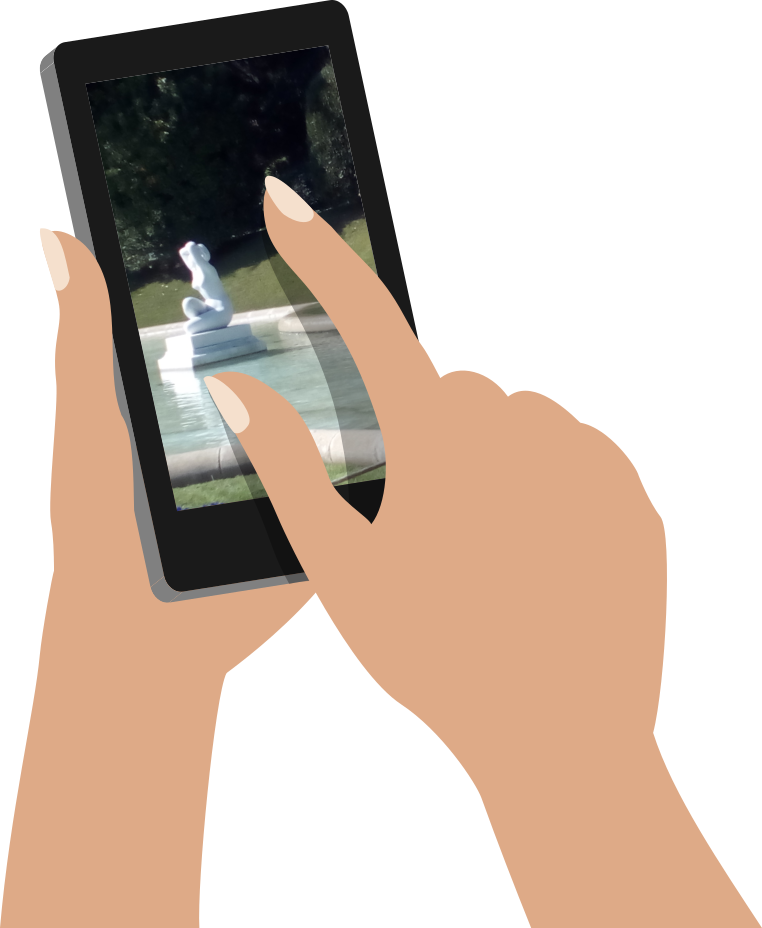
\includegraphics[width=0.6\textwidth]{images/smartjardi}
			\end{figure}
		\end{minipage}
		\hfill
		\begin{minipage}{0.49\textwidth}
			\begin{enumerate}
				\item Selecció de l'usuari
				\item Captura del robot
				\item Localització
				\item Desplaçament
			\end{enumerate}
		\end{minipage}
	\end{frame}

	\begin{frame}[plain]
		\section{Planificació}
	\end{frame}

	% TASQUES
	\begin{frame}{Tasques (blocs)}
		\tz
		\begin{table}[H]
			\begin{center}
				\adjustbox{max width=\textwidth}{
				\rowcolors{2}{myOrange}{}
				\begin{tabular}{l !{\vrule width -1pt}c !{\vrule width -1pt}r}
					\textbf{Descripció} & \textbf{Metodologia} & \textbf{Hores} \\ \hline
					Preparació de l'entorn & - & 5h \\
					Curs de GEP & Cascada & 75h \\
					Desenvolupament del projecte & Àgil & 355h \\
					Preparació de la defensa & - & 45h \\
				\end{tabular}
				}
			\end{center}
			\caption{Blocs del projecte}
		\end{table}
	\end{frame}

	% DESENVOLUPAMENT
	\begin{frame}{Tasques (desenvolupament)}
		\tz
		\centering
		\begin{figure}
			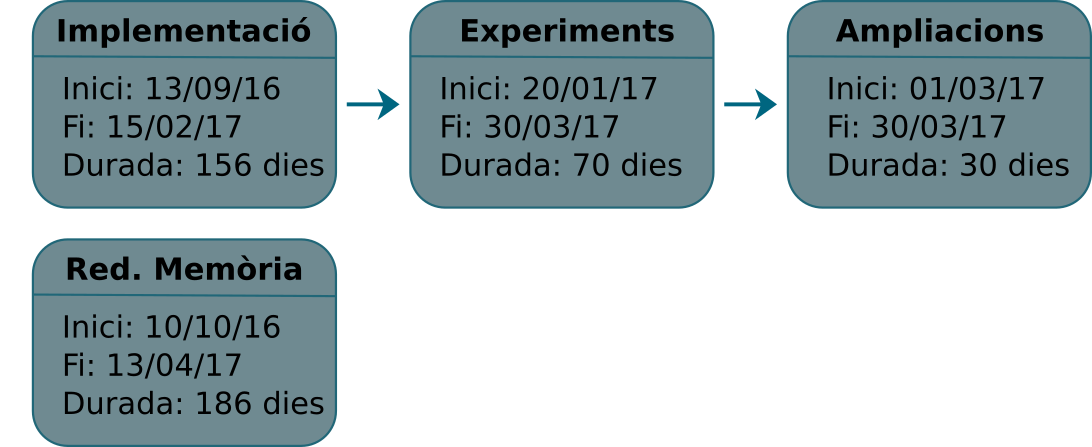
\includegraphics[width=\textwidth-0.2cm]{images/tasques}
			\vspace{0.2cm}
			\caption{Tasques desenvolupament}
		\end{figure}
	\end{frame}

	% GANTT
	\begin{frame}{Diagrama de Gantt}
		\tz
		\centering
		\begin{figure}
			\makebox[\textwidth][c]{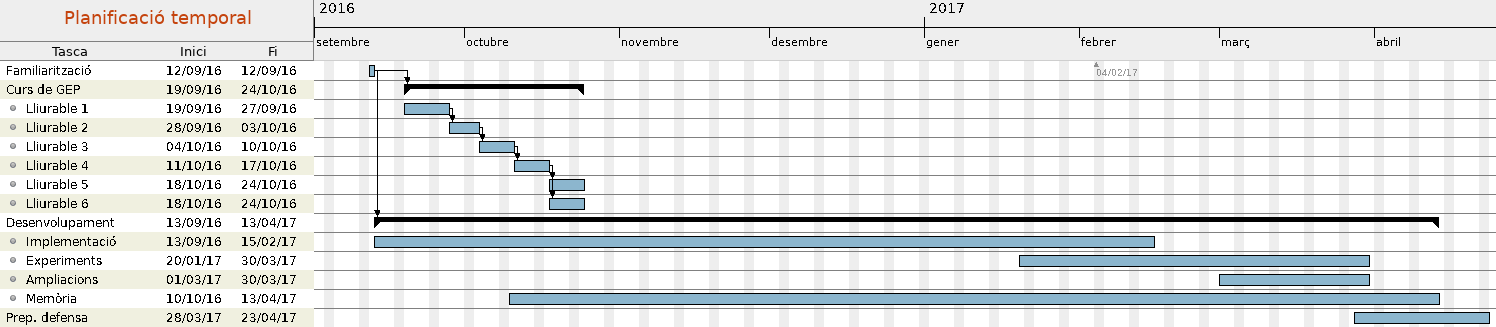
\includegraphics[width=1.1\textwidth]{images/gantt}}%
			\vspace{0.2cm}
			\caption{Gantt del projecte}
		\end{figure}
	\end{frame}

	\begin{frame}[plain]
		\section{Gestió econòmica i sostenibilitat}
	\end{frame}

	% HARDWARE
	\begin{frame}{Maquinari}
		\tz
		\begin{table}[H]
			\begin{center}
				\begin{tabular}{l !{\vrule width -1pt}r !{\vrule width -1pt}r !{\vrule width -1pt}r !{\vrule width -1pt}r}
					\textbf{Producte} & \textbf{Preu} & \textbf{Ús} & \textbf{Vida útil} & \textbf{Amortització} \\ \hline
					Ordinador & 500€ & 7 mesos & 5 anys & 58,33€ \\
					Smartphone & 39€ & 1 mes & 3 anys & 1,08€ \\
					\noalign{\vskip 4mm}
					\rowcolor{total}
					Total &  &  &  & 59,41€ \\
				\end{tabular}
			\end{center}
			\caption{Recursos de maquinari}
		\end{table}
	\end{frame}

	% SOFTWARE
	\begin{frame}{Programari}
		\begin{table}[H]
			\begin{center}
			\adjustbox{max width=\textwidth}{
				\rowcolors{2}{myOrange}{white}
				\begin{tabular}{l !{\vrule width -1pt}p{5cm} !{\vrule width -1pt}p{5cm}}
				\textbf{Nom} & \textbf{Tipus} & \textbf{Ús} \\ \hline
				Arch Linux/Raspbian & Eina de desenvolupament & Execució del programari \\
				Python + OpenCV & Eina de desenvolupament & Programació \\
				Flask & Eina de desenvolupament & Micro-framework \\
				uWSGI & Eina de desenvolupament & Servidor uwsgi \\
				Nginx & Eina de desenvolupament & Servidor web/proxy \\
				Geany/Atom & Eina de desenvolupament & Programació del codi \\
				\LaTeX & Documentació & Redacció de la memòria \\
				Zathura & Documentació & Visualització de pdf \\
				Gantt Project & Eina de gestió & Creació diagrames de Gantt \\
				Git + GitHub & Desenvolupament i gestió & Control de versions \\
				\end{tabular}
			}
			\end{center}
			\caption{Recursos de programari}
		\end{table}
	\end{frame}

	% RECURSOS HUMANS
	\begin{frame}{Recursos humans I}
		\begin{table}[H]
			\centering
			\adjustbox{max width=\textwidth, max height=\dimexpr\textheight-5.52cm\relax}{
				\begin{tabular}{l !{\vrule width -1pt}c !{\vrule width -1pt}c !{\vrule width -1pt}c}
					\textbf{Tasca} & \textbf{Cap de projecte} & \textbf{Analista} & \textbf{Programador} \\ \hline
					Preparació de l'entorn & 3h & & 2h \\
					Curs de GEP & 75h & & \\
					Implementació i proves & & 30h & 195h \\
					Experiments & & & 40h \\
					Ampliacions & & 10h & 30h\\
					Redacció memòria & 50h & & \\
					Preparació defensa & 45h & & \\
					\noalign{\vskip 4mm}
					\rowcolor{total}
					Total & 173h & 40h & 267h
				\end{tabular}
			}
			\caption{Recursos humans (hores)}
		\end{table}
	\end{frame}
	
	% RECURSOS HUMANS II
	\begin{frame}{Recursos humans II}
		\tz
		\begin{table}[H]
			\centering
			\adjustbox{max width=\textwidth}{
				\begin{tabular}{l !{\vrule width -1pt}r !{\vrule width -1pt}r !{\vrule width -1pt}r}
					\textbf{Rol} & \textbf{Hores} & \textbf{Cost/hora} & \textbf{Cost total} \\ \hline
					Cap de projecte & 173h & 25€/h & 4325€ \\
					Analista & 40h & 20€/h & 800€ \\
					Programador & 267h & 15€/h & 4005€ \\
					\noalign{\vskip 4mm}
					\rowcolor{total}
					Total & & & 9130€
				\end{tabular}
			}
			\caption{Recursos humans (costos)}
		\end{table}
	\end{frame}

	%\begin{frame}{Costos indirectes}
	%	\tz
	%	\begin{table}[H]
	%		\begin{center}
	%			\begin{tabular}{l !{\vrule width -1pt}r !{\vrule width -1pt}r !{\vrule width -1pt}r}
	%				\textbf{Tipus} & \textbf{Temps} & \textbf{Cost} & \textbf{Cost total} \\ \hline
	%				Electricitat* & 480h & 0,028€/h & 13,44€ \\
	%				Accès a Internet & 480h & 0,17€/h & 81,6€ \\
	%				\noalign{\vskip 4mm}
	%				\rowcolor{total}
	%				Total & & & 95,04€
	%			\end{tabular}
	%		\end{center}
	%		\caption{Costos indirectes}
	%	\end{table}
	%	\tiny{* Cost de l'electricitat = 0,141033€/kWh (considerem la potència 0,2kW)}
	%\end{frame}

	% COSTOS
	\begin{frame}{Costos totals}
		\begin{table}[H]
			\begin{center}
			\adjustbox{max width=\textwidth}{
				\begin{tabular}{p{8cm}  !{\vrule width -1pt}r}
					\textbf{Tipus} & \textbf{Cost estimat} \\ \hline
					Recursos humans & 9.130€ \\
					Recursos de programari & 0€ \\
					Recursos de maquinari & 59,41€ \\
					Costos indirectes & 95,04€ \\
					Imprevistos & 600€ \\
					Contingència (5\%) & 494,22€ \\
					\noalign{\vskip 4mm}
					\rowcolor{total}
					Total & 10.378,67€
				\end{tabular}
			}
			\end{center}
			\caption{Costos totals}
		\end{table}
	\end{frame}

% SOSTENIBILITAT
%\section{Lleis i sostenibilitat}

%	\begin{frame}{Lleis i regulacions}
%		\tz
%		Caldrà tenir en compte les lleis i regulacions, tant a l'hora de realitzar el projecte com a l'hora de publicar-lo o fer la documentació.\\
%		\vspace{1em}
%		\begin{itemize}
%			\item Drets d'imatge
%			\item Patents dels algorismes
%			\item Drets d'autor
%		\end{itemize}
%	\end{frame}

	\begin{frame}{Sostenibilitat}
		\tz
		\begin{table}[H]
			\begin{center}
			\adjustbox{max width=\textwidth}{
				\begin{tabular}{l !{\vrule width -1pt}M{3.7cm} !{\vrule width -1pt}M{3.4cm} !{\vrule width -1pt}M{3.4cm}}
					\textbf{Sostenibilitat} & \textbf{PPP} & \textbf{Vida útil} & \textbf{Riscos} \\ \hline
					Ambiental & \bigcell{c}{Consum del disseny \\ {\textbf{8} [0:10]}} & \bigcell{c}{Petjada ecològica \\ {\textbf{15} [0:20]}} & \bigcell{c}{Riscos ambientals \\ {\textbf{0} [-20:0]}} \\
					\noalign{\vskip 2mm}
					Econòmica & \bigcell{c}{Factura \\ {\textbf{7} [0:10]}} & \bigcell{c}{Pla de viabilitat \\ {\textbf{10} [0:20]}} & \bigcell{c}{Riscos econòmics \\ {\textbf{0} [-20:0]}} \\
					\noalign{\vskip 2mm}
					Social & \bigcell{c}{Impacte personal \\ {\textbf{8} [0:10]}} & \bigcell{c}{Impacte social \\ {\textbf{5} [0:20]}} & \bigcell{c}{Riscos socials \\ {\textbf{0} [-20:0]}} \\
					\noalign{\vskip 4mm}
					\rowcolor{myBlue}
					Valoració total & \multicolumn{3}{c}{\textbf{53} [-60:90]} \\
				\end{tabular}
			}
			\end{center}
			\caption{Matriu de sostenibilitat}
		\end{table}
	\end{frame}

	\begin{frame}[plain]
		\section{Arquitectura del sistema}
	\end{frame}

	% ARQUITECTURA
	\begin{frame}{Arquitectura del sistema}
		\tz
		\centering
		\begin{figure}
			
\includegraphics[width=0.6\textwidth]{images/arquitectura}
			\vspace{0.2cm}
			\captionsource{Arquitectura del sistema}{Madebyoliver i Freepik}
		\end{figure}
	\end{frame}

	% APLICACIÓ
	\begin{frame}{Aplicació - Disseny}
		\tz
		\centering
		\begin{figure}[H]
			\resizebox{\textwidth}{!}{%
			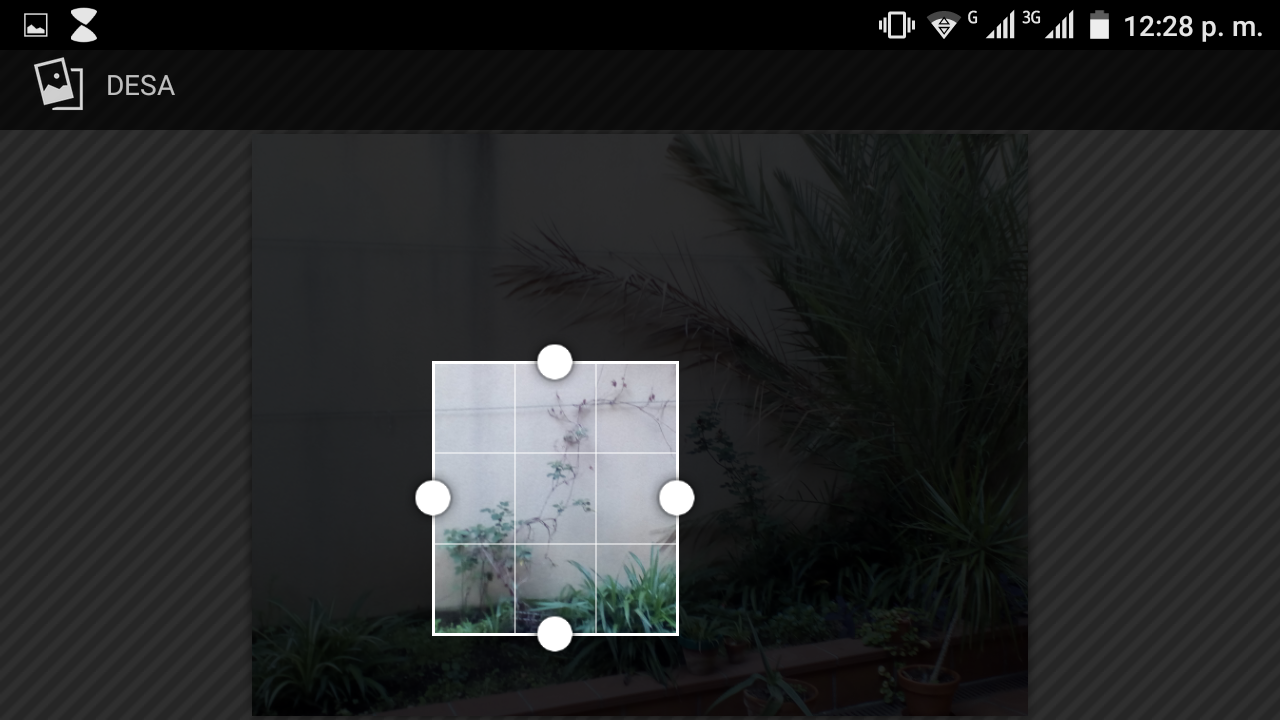
\includegraphics[height=1cm]{images/crop}
			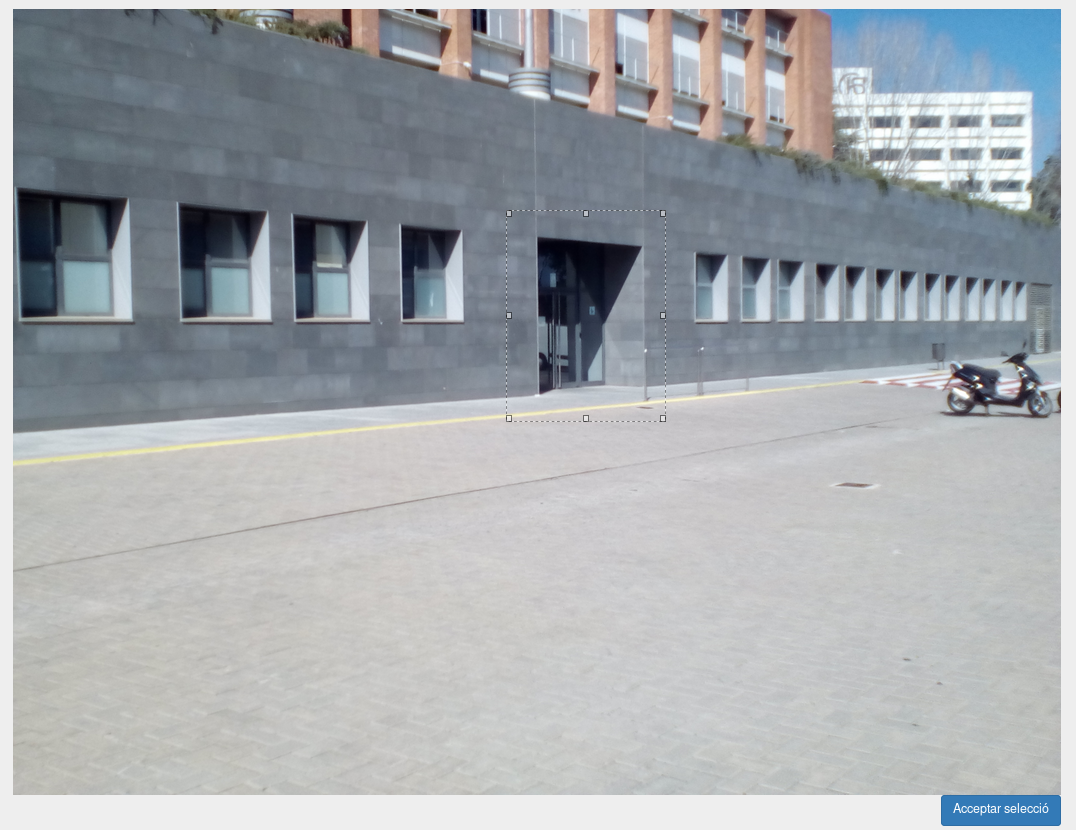
\includegraphics[height=1cm]{images/webapp}}
			\caption{Selecció de la regió d'interès}
		\end{figure}
	\end{frame}

	%\begin{frame}{Aplicació - Disseny II}
	%	\centering
	%	\begin{figure}[!htb]
	%		\resizebox{\textwidth}{!}{%
	%		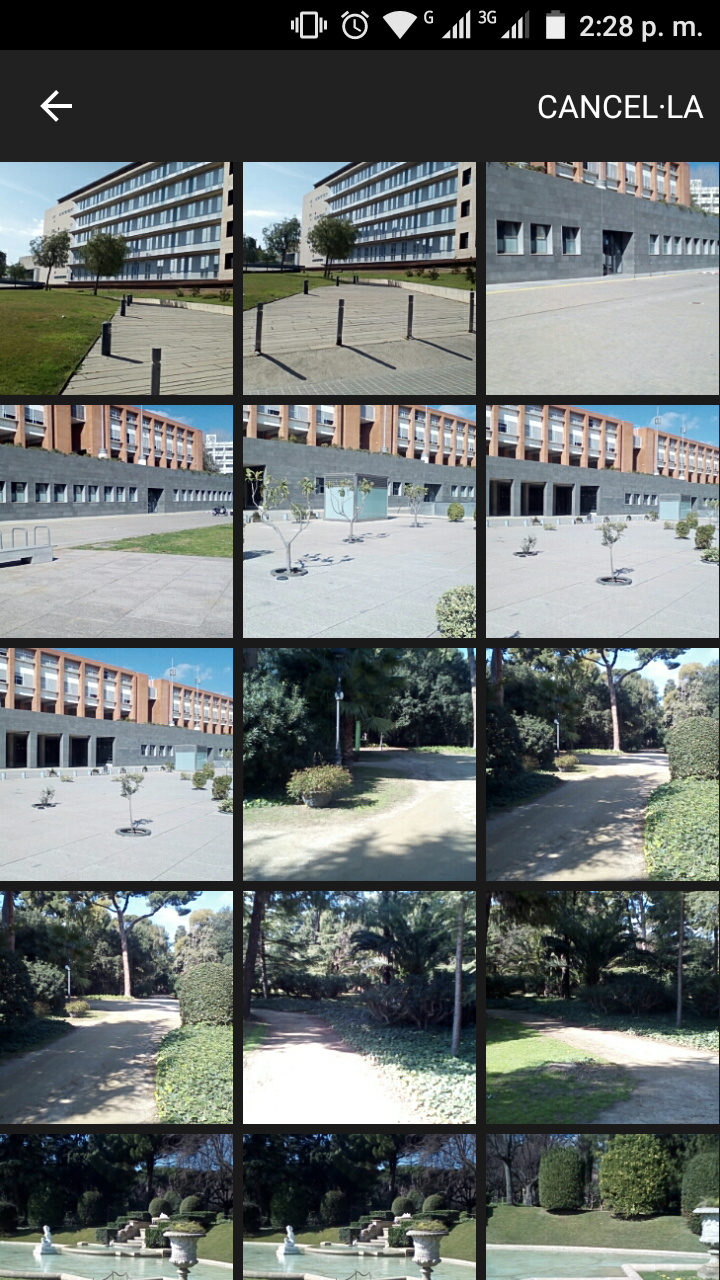
\includegraphics[height=1cm]{images/gallery}
	%		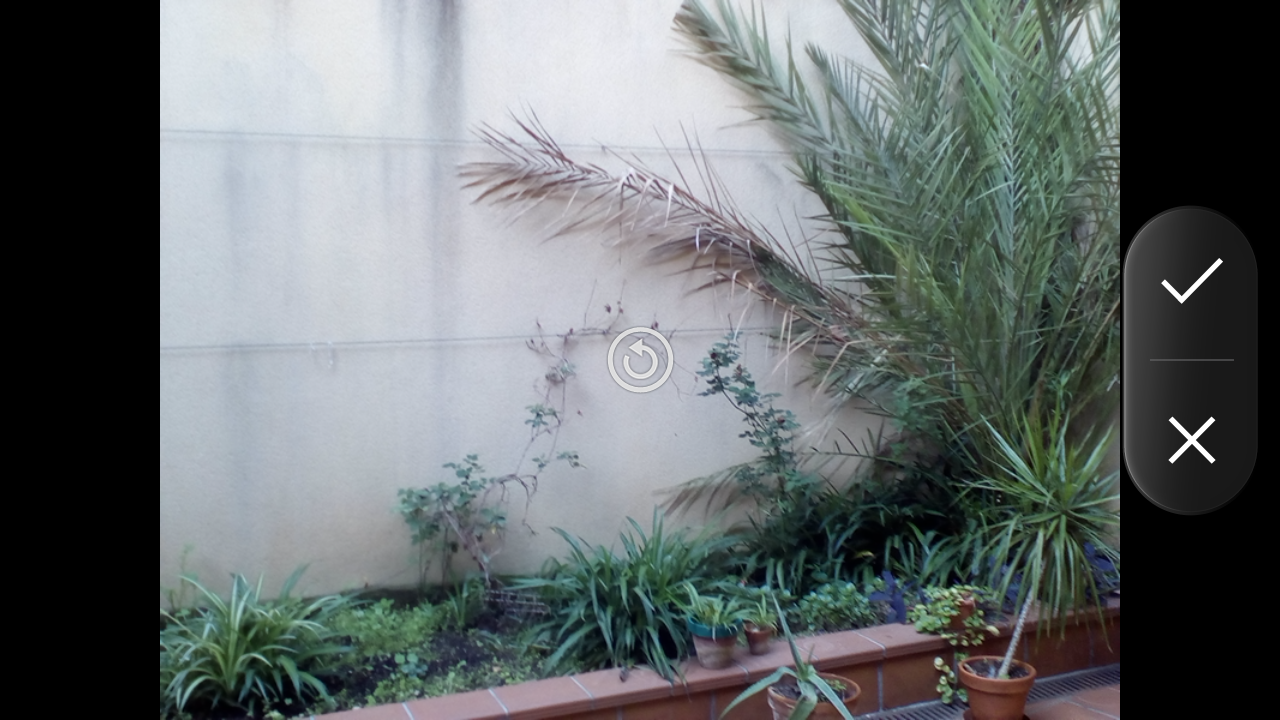
\includegraphics[height=1cm]{images/cam}}
	%		\caption{Selecció de la regió d'interès}
	%	\end{figure}
	%\end{frame}

	% SERVIDOR
	\begin{frame}{Servidor - Estructura}
		\tz
		\centering
		\begin{figure}
			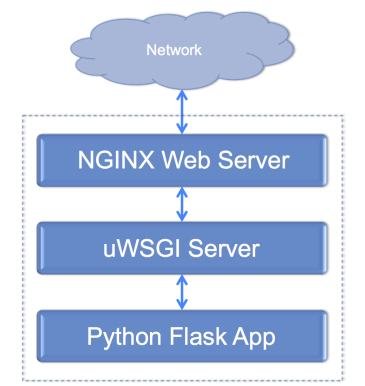
\includegraphics[width=0.4\textwidth]{images/server}
			\vspace{0.2cm}
			\captionsource{Estructura del servidor}{https://iotbytes.wordpress.com}
		\end{figure}
	\end{frame}

	\begin{frame}{Servidor - Instal·lació}
		\tz
		\begin{enumerate}
			\item{Instal·lar el sistema operatiu}
			\item{Instal·lar Python + OpenCV}
			\item{Instal·lar Flask}
			\item{Instal·lar uWSGI i Nginx}
			\item{Configuració bàsica}
		\end{enumerate}
	\end{frame}

%	\begin{frame}{Servidor - Configuració}
%		\tz
%		\metroset{block=fill}
%		\begin{alertblock}{Flask}
%			Simmons Hall is composed of metal and concrete.
%		\end{alertblock}
%		\begin{alertblock}{uWSGI}
%			Simmons Hall is composed of metal and concrete.
%		\end{alertblock}
%		\begin{alertblock}{Nginx}
%			Simmons Hall is composed of metal and concrete.
%		\end{alertblock}
%	\end{frame}

% TÈCNIQUES UTILITZADES
	\begin{frame}[plain]
		\section{Tècniques de visió utilitzades}
	\end{frame}

	\begin{frame}{Tècniques de visió}
		\tz
		\begin{enumerate}
			\item Preprocessat digital d'imatges
			\item Detecció de punts d'interès
			\item Extracció de característiques
			\item \textit{Matching} de característiques
			\item Homografia
		\end{enumerate}
	\end{frame}

	\begin{frame}{Detecció de keypoints}
		\tz
		\metroset{block=fill}
		\begin{block}{Què és?}
			Consisteix a obtenir punts de la imatge amb característiques distintives, que ens puguin ser útils més endavant.
		\end{block}
		Algorismes principals utilitzats:
		\begin{itemize}
			\item Harris\cite{Harris}
			\item SIFT\cite{SIFT}
			\item ORB\cite{Rublee:2011:OEA:2355573.2356268}
		\end{itemize}
	\end{frame}

	\begin{frame}{Harris I}
		\tz
		\begin{minipage}{0.53\textwidth}
			\begin{itemize}
				\item Detector de cantonades
				\item Finestra NxM píxels
				\item Busca canvis d'intensitat
				\item \alert{No és invariant a l'escala}
			\end{itemize}
		\end{minipage}
		\hfill
		\begin{minipage}{0.45\textwidth}
			\begin{figure}[H]
				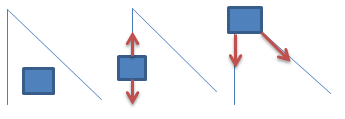
\includegraphics[width=\textwidth]{images/harris}
				\captionsource{Pla, vora i cantonada\vspace{0.1cm}}{Wikipedia}
			\end{figure}
		\end{minipage}
	\end{frame}

	\begin{frame}{Harris II}
		\tz
		S'ha optat per aplicar Harris en diverses escales, fent una piràmide de la imatge original. A cada nivell, es redueix la imatge a la meitat.
		\begin{figure}[H]
			\centering
			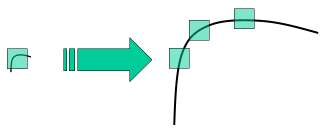
\includegraphics[width=0.5\textwidth]{images/scale_invariant}
			\captionsource{\textit{Cantonada a diferent escala}}{OpenCV}
			\label{fig:vores}
		\end{figure}
	\end{frame}

	\begin{frame}{SIFT - Detector I}
		\tz
		\begin{enumerate}
			\item{Diferència de Gaussianes en diferents escales}
			\item{Màxims i mínims locals en l'espai i l'escala}
			\item{Es repeteixen els passos fent una piràmide}
			\newcounter{enumTemp}
			\setcounter{enumTemp}{\theenumi}
		\end{enumerate}
		\begin{figure}[H]
			\resizebox{0.8\textwidth}{!}{%
			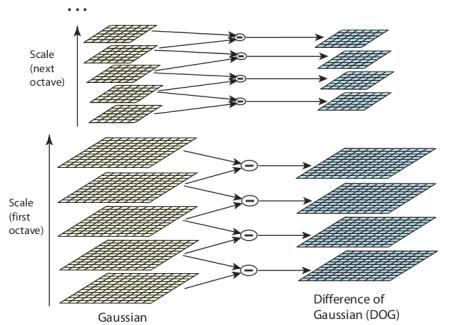
\includegraphics[height=1cm]{images/sift_dog}
			\hfill
			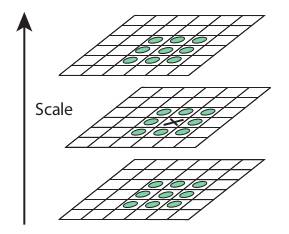
\includegraphics[height=1cm]{images/sift_local_extrema}}
			\captionsource{\textit{SIFT - DoG i \textit{local extrema}}}{OpenCV}
		\end{figure}
	\end{frame}

	\begin{frame}{SIFT - Detector II}
		\tz
		\begin{enumerate}
			\setcounter{enumi}{\theenumTemp}
			\item{S'eliminen punts amb intensitat menor a un cert llindar}
			\item{S'eliminen vores}
			\item{S'assigna una orientació als punts}
		\end{enumerate}
	\end{frame}

	\begin{frame}{ORB - Detector I}
		\tz
		\begin{itemize}
			\item{Detector FAST\cite{Rosten:2006:MLH:2094437.2094478} amb modificacions}
			\item{Detecció de cantonades, molt ràpid}
			\item{Es compara la intensitat d'un píxel amb N veïns}
		\end{itemize}
		\begin{figure}[H]
			\centering
			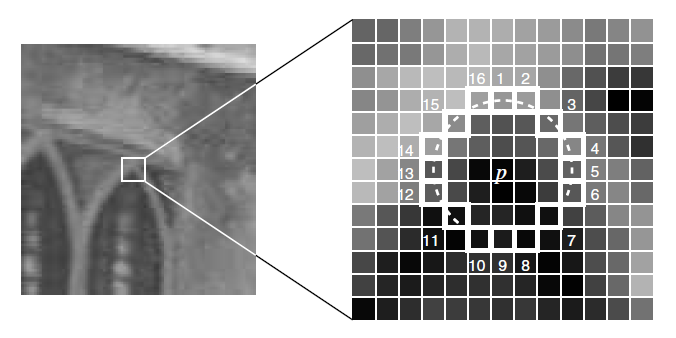
\includegraphics[width=0.55\textwidth]{images/fast}
			\captionsource{FAST, N=16}{https://www.edwardrosten.com/work/fast.html}
		\end{figure}
		%Suposant que N = 16 i definint un llindar t, si 12 píxels veïns (\sfrac{3}{4} parts) són majors a I\textsubscript{p} + t o bé menors a I\textsubscript{p} - t, es considera que el punt és d'interès.
		%El problema principal de FAST és que no té en compte l'orientació.\\\\
	\end{frame}

	\begin{frame}{ORB - Detector II}
		\tz
		\alert{FAST no és invariant a l'escala ni la rotació.}\\
		\vspace{0.5cm}
		ORB aplica les següents millores:\\

		\begin{itemize}
			\item{S'agafen els N millors punts, aplicant la mesura de Harris.}
			\item{Es fa una piràmide per fer multi-escala.}
			\item{S'utilitzen els moments per calcular l'orientació.}
		\end{itemize}
	\end{frame}

	\begin{frame}{Extracció de característiques}
		\tz
		\metroset{block=fill}
		\begin{block}{Què és?}
			Consisteix en descriure característiques de les imatges en els punts donats. Podrem comparar aquestes característiques amb les d'una altre imatge i veure si són similars.
		\end{block}
		Algorismes principals utilitzats:
		\begin{itemize}
			\item SIFT
			\item ORB
			\item BRISK\cite{Leutenegger:2011:BBR:2355573.2356277}
		\end{itemize}
	\end{frame}

	\begin{frame}{SIFT - Descriptor}
		\tz
		\begin{itemize}
			\item Veïnatge de 16x16 píxels al voltant del punt
			\item Divisió en 16 blocs de 4x4
			\item Per cada sub-bloc es calcula histograma d'orientacions en 8 direccions (vector de dimensió 128)
		\end{itemize}
		\begin{figure}[H]
			\centering
			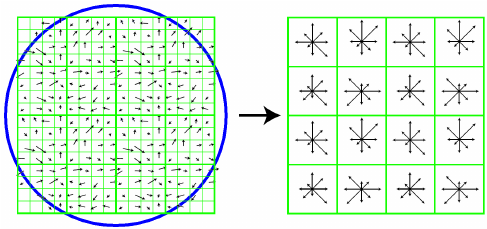
\includegraphics[width=0.6\textwidth]{images/sift-des}
			\captionsource{Descriptor SIFT}{https://www.researchgate.net}
		\end{figure}
	\end{frame}

	\begin{frame}{ORB - Descriptor}
		\tz
		\begin{itemize}
			\item Descriptor binari, senzill i ràpid
			\item Modificació BRIEF\cite{Calonder:2010:BBR:1888089.1888148}
			\item N parells de píxels veïns
			\item Per cada parell es compara la intensitat i es retorna 1 o 0 segons si és major la del primer o la del segon
			\item \alert{BRIEF no és invariable en la rotació} \textrightarrow{} ORB ``gira'' el patró en funció de l'angle
		\end{itemize}
	\end{frame}

	\begin{frame}{BRISK}
		\tz
		\begin{minipage}{0.53\textwidth}
			\begin{itemize}
				\item Descriptor binari
				\item Patró de cercles concèntrics
				\item Comparació cadenes binàries amb XOR
			\end{itemize}
		\end{minipage}
		\hfill
		\begin{minipage}{0.45\textwidth}
			\begin{figure}[H]
				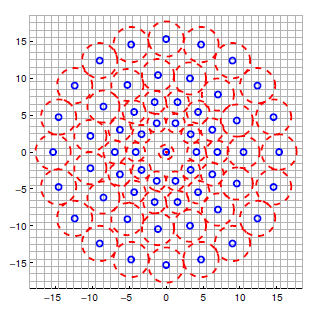
\includegraphics[width=0.9\textwidth]{images/brisk}
				\captionsource{Patró BRISK\vspace{0.1cm}}{https://gilscvblog.com}
			\end{figure}
		\end{minipage}
	\end{frame}

	\begin{frame}{Matching}
		\tz
		\begin{minipage}{0.62\textwidth}
			\metroset{block=fill}
			\begin{block}{Què és?}
				Consisteix en trobar coincidències entre els punts de dues imatges, comparant les seves característiques.\par
				Pels descriptors binaris utilitzem la distància de Hamming i pels vectorials l'euclidiana.
			\end{block}
		\end{minipage}
		\hfill
		\begin{minipage}{0.36\textwidth}
			\begin{figure}[H]
				\vspace{0.8cm}
				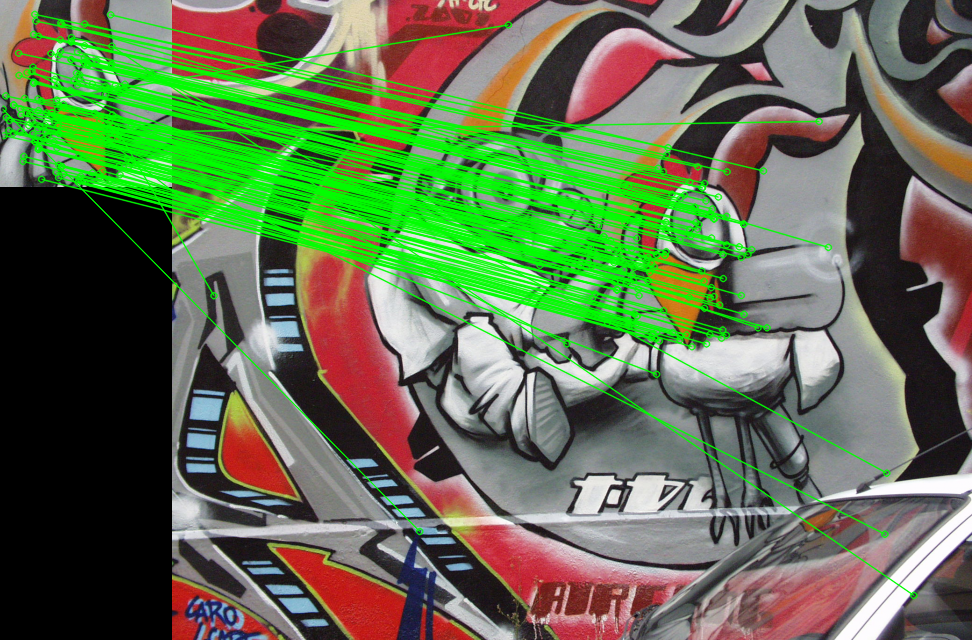
\includegraphics[width=\textwidth]{images/matching}
				\caption{\textit{Matching}}
			\end{figure}
		\end{minipage}
	\end{frame}

	\begin{frame}{Homografia I}
		\tz
		\begin{minipage}{0.62\textwidth}
			\metroset{block=fill}
			\begin{block}{Què és?}
				Trobant la relació entre els píxels de les dues imatges podrem reprojectar el pla d'una imatge en l'altre i trobar el punt on volem dirigir el robot.
			\end{block}
		\end{minipage}
		\hfill
		\begin{minipage}{0.36\textwidth}
			\begin{figure}[H]
				\vspace{0.8cm}
				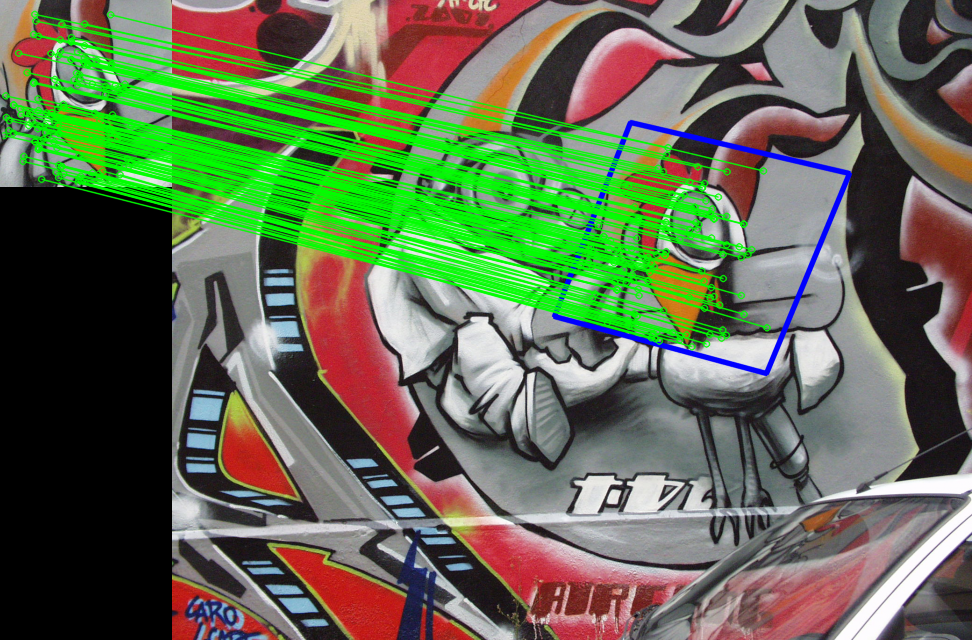
\includegraphics[width=\textwidth]{images/homography}
				\caption{\textit{Homografia}}
			\end{figure}
		\end{minipage}
	\end{frame}

	\begin{frame}{Homografia II}
		Aplicarem RANSAC (\textit{Random Sample Consensus})\cite{Fischler:1981:RSC:358669.358692},
		un algorisme que ens permetrà eliminar \textit{outliers}.
		\begin{figure}[H]
			\centering
			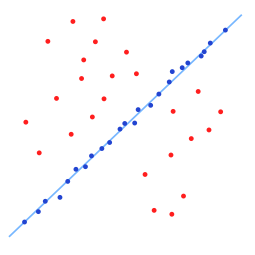
\includegraphics[width=0.3\textwidth]{images/ransac}
			\captionsource{RANSAC}{Wikipedia}
		\end{figure}
	\end{frame}

%RESULTATS

	\begin{frame}[plain]
		\section{Resultats}
	\end{frame}

	\begin{frame}{Imatges similars I}
		\tz
		\begin{figure}[!htb]
			\minipage{0.4\textwidth}
				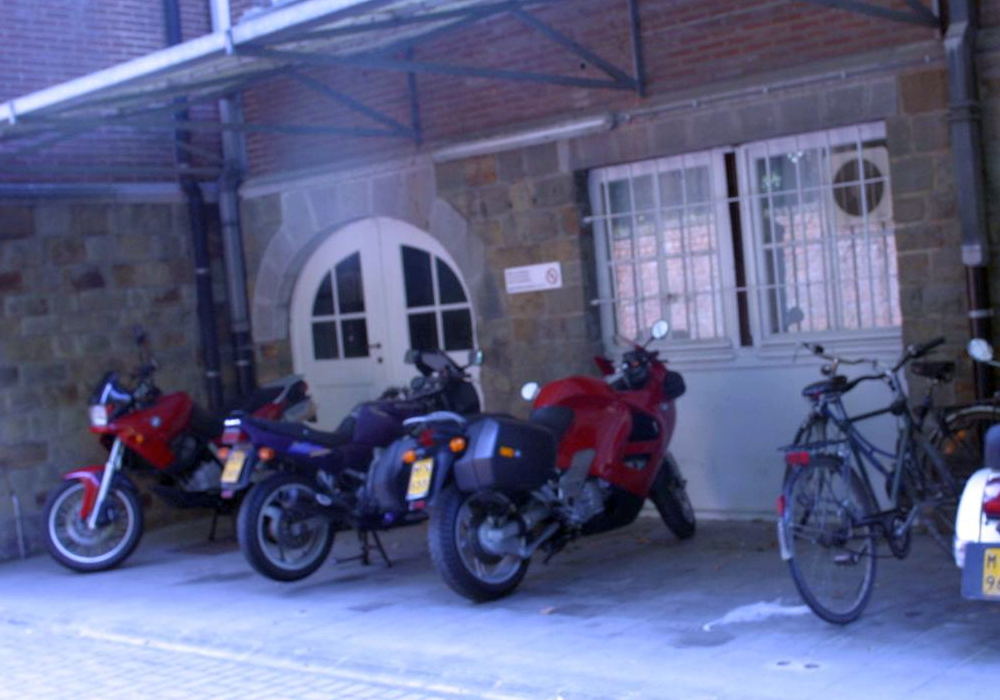
\includegraphics[width=\linewidth]{images/experiments/motos3}
			\endminipage
			\hspace*{0.2cm}
			\minipage{0.4\textwidth}
				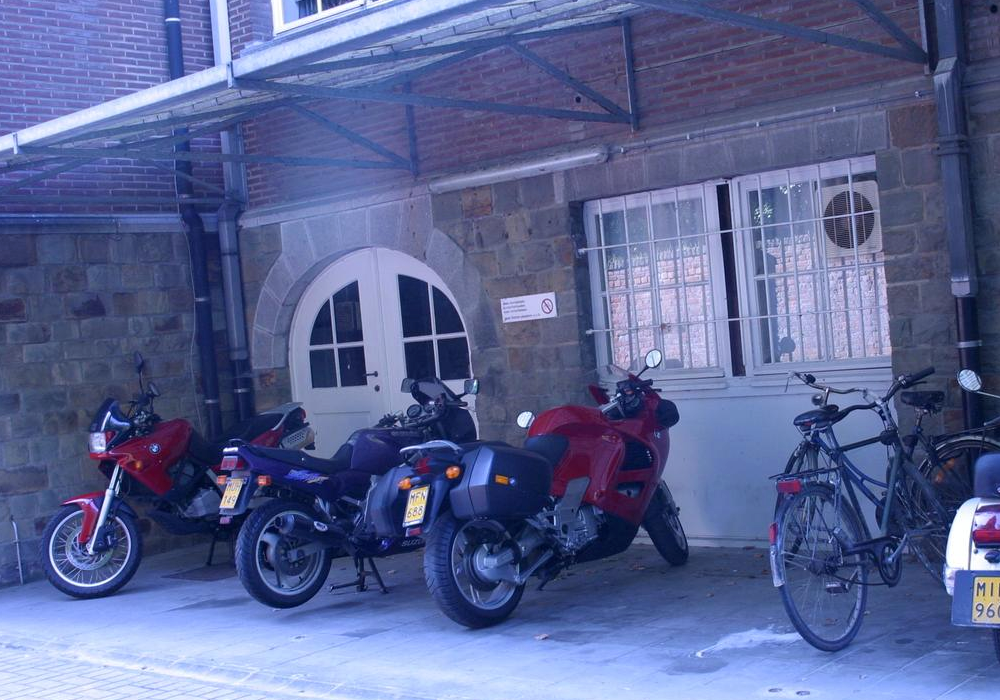
\includegraphics[width=\linewidth]{images/experiments/motos1}
			\endminipage

			\minipage{0.4\textwidth}
				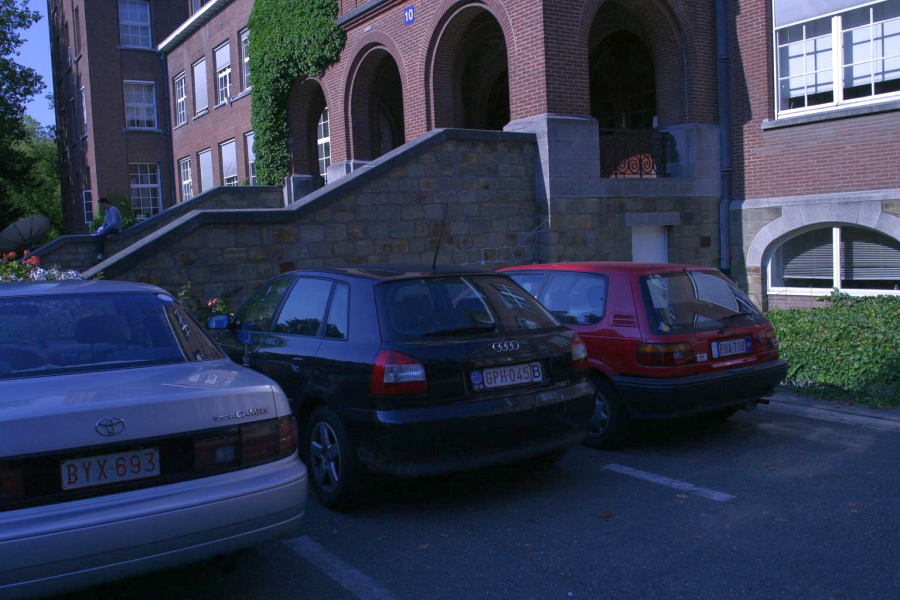
\includegraphics[width=\linewidth]{images/experiments/cars4}
			\endminipage
			\hspace*{0.2cm}
			\minipage{0.4\textwidth}
				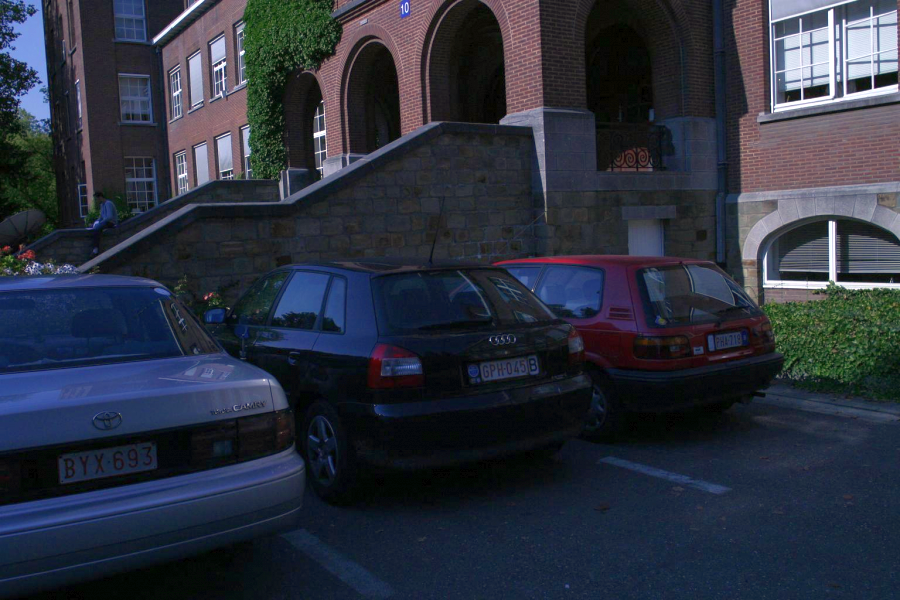
\includegraphics[width=\linewidth]{images/experiments/cars6}
			\endminipage
			\caption{Imatges motos i cotxes}
		\end{figure}
	\end{frame}

	\begin{frame}{Imatges similars II}
		\tz
		\begin{table}[H]
			\begin{center}
				\rowcolors{3}{}{myBlue}
				\adjustbox{max width=\textwidth}{
				\begin{tabular}{l | c c | c c}
					& \multicolumn{2}{c|}{\textbf{Motos}} & \multicolumn{2}{c}{\textbf{Cotxes}} \\
					\textbf{Algorismes} & \textbf{Correctes} & \textbf{Erronis} & \textbf{Correctes} & \textbf{Erronis} \\ \hline
					Harris + SIFT & 110 & 1 & 98 & 4 \\
				\end{tabular}
				}
			\end{center}
			\caption{\textit{Matching} - imatges similars}
		\end{table}
	\end{frame}

	\begin{frame}{Objectes I}
		\tz
		\begin{figure}[H]
			\resizebox{0.6\textwidth}{!}{%
			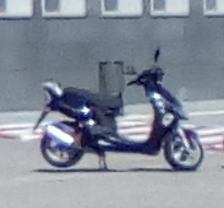
\includegraphics[height=1cm]{images/experiments/uni_sel}
			%\hspace{0.1cm}
			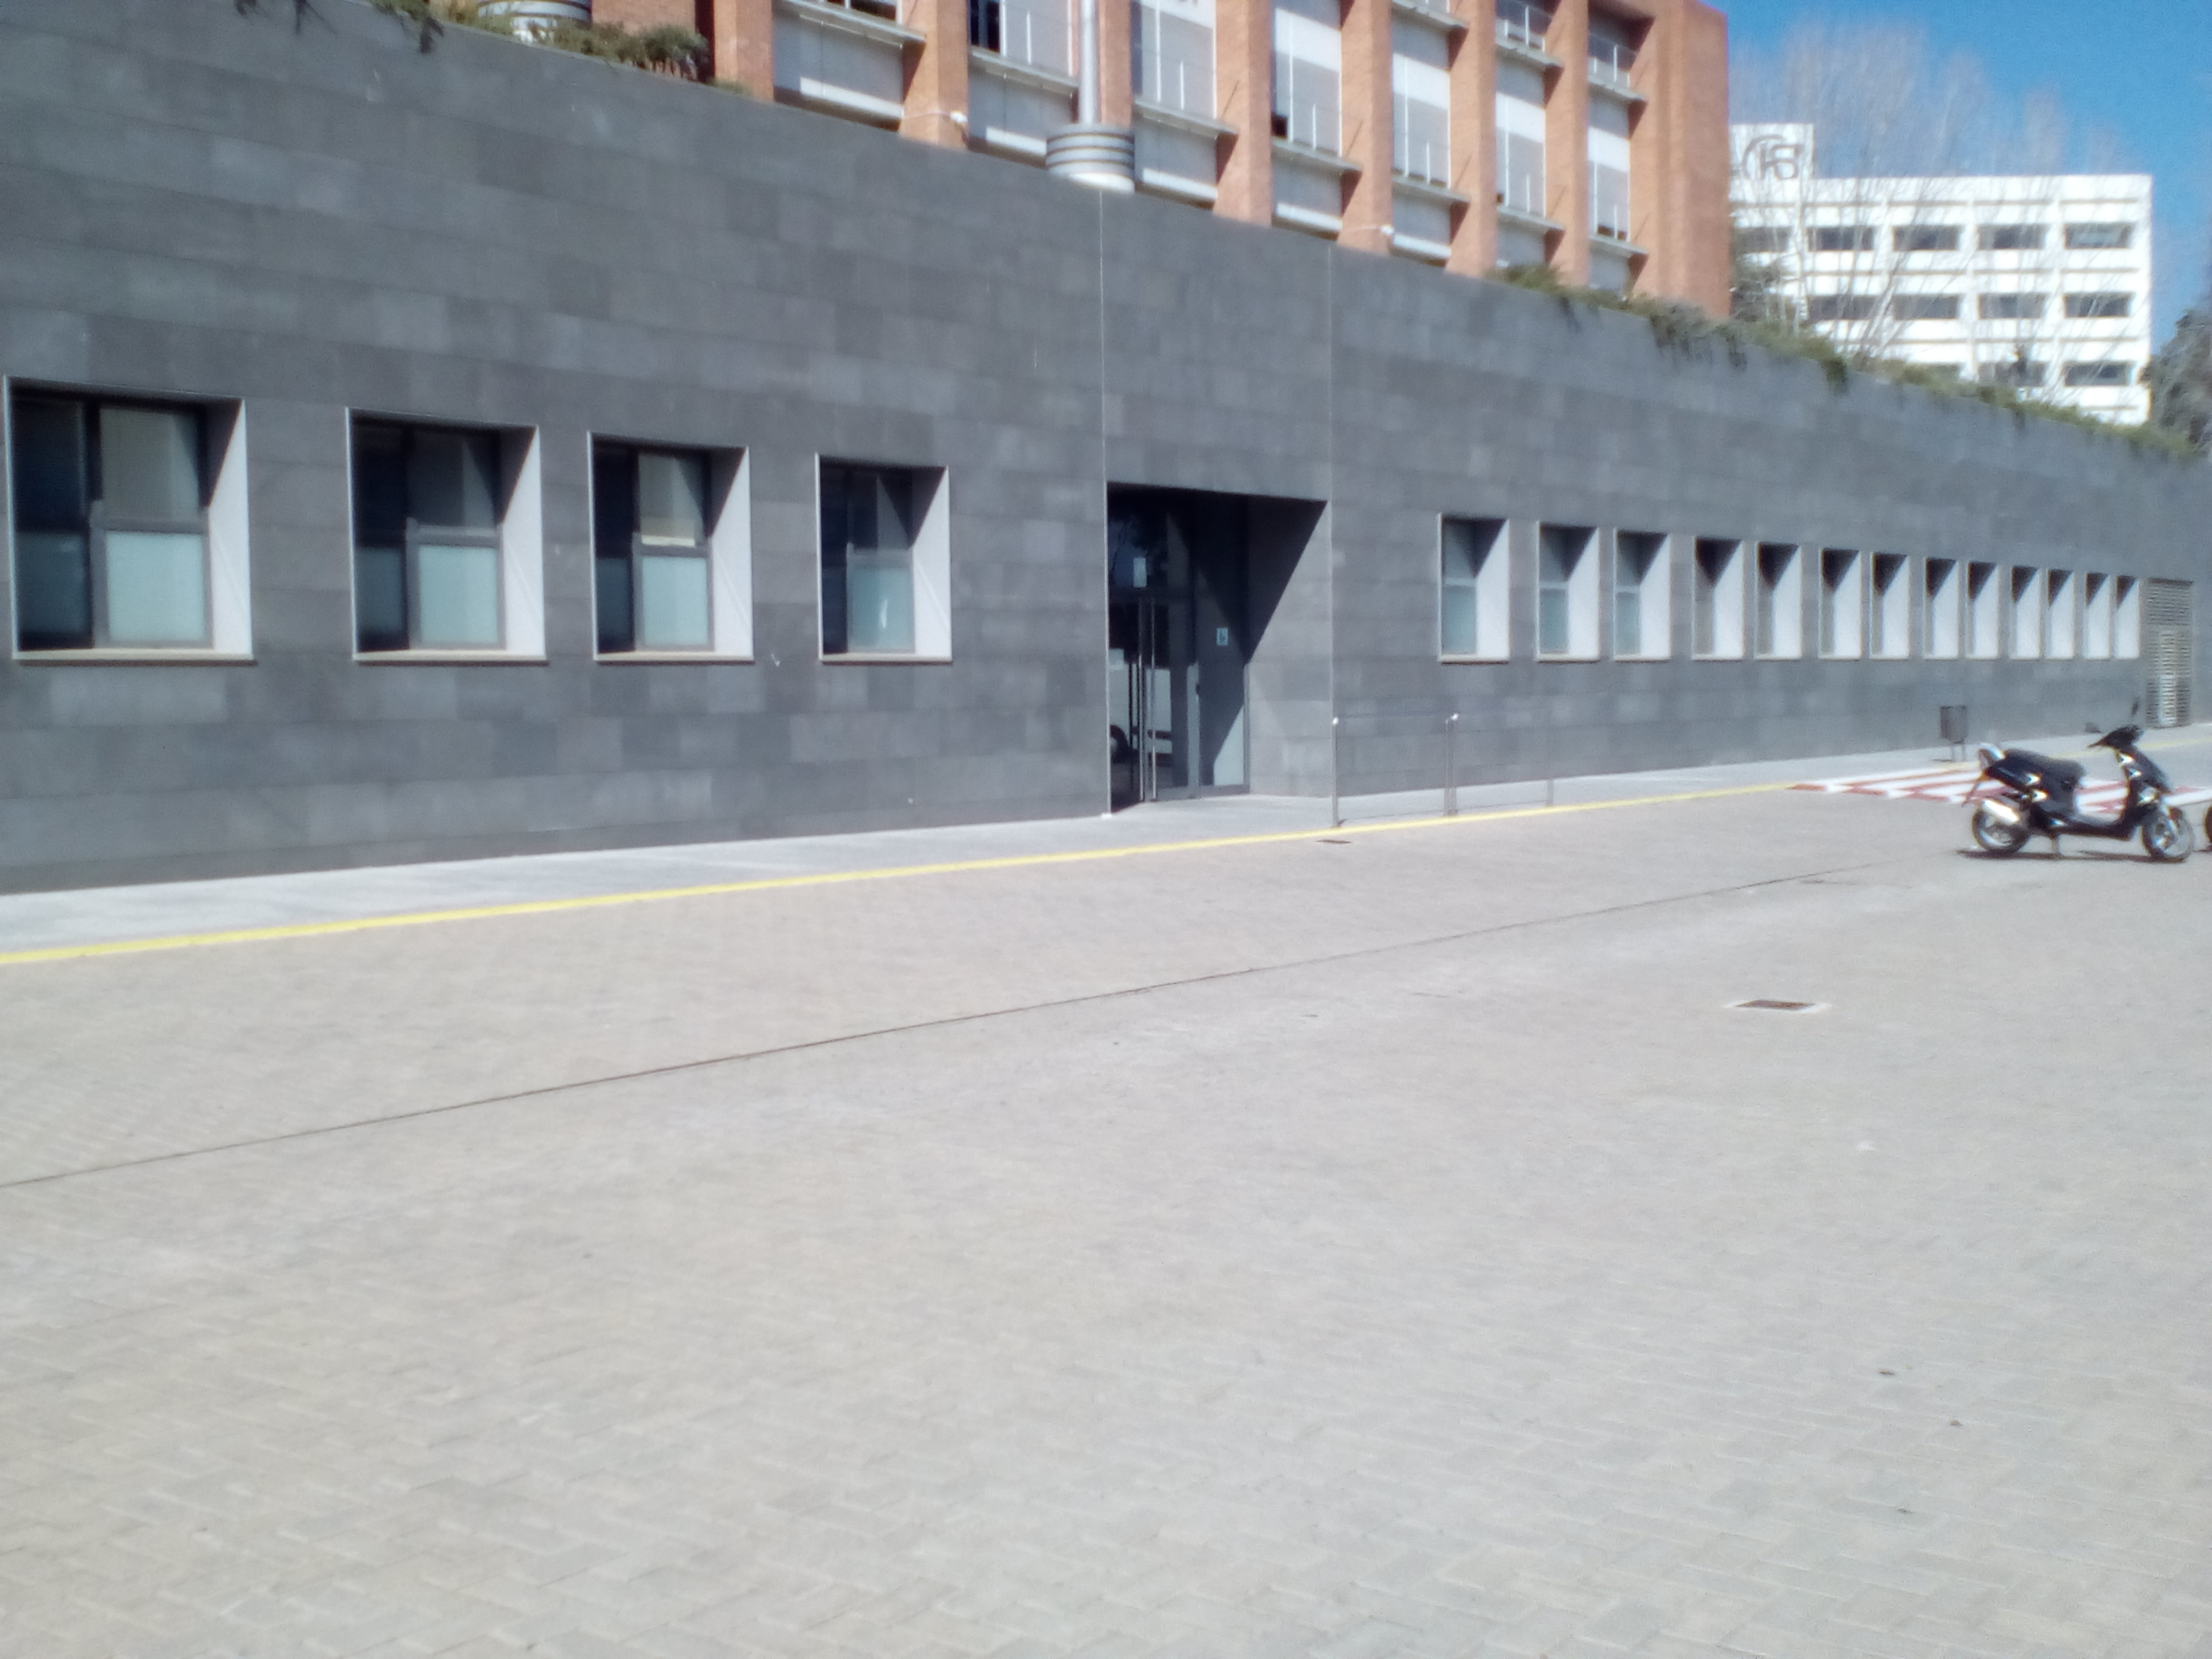
\includegraphics[height=1cm]{images/experiments/uni1}}
			%\vspace*{2cm}
			\par
			\resizebox{0.6\textwidth}{!}{%
			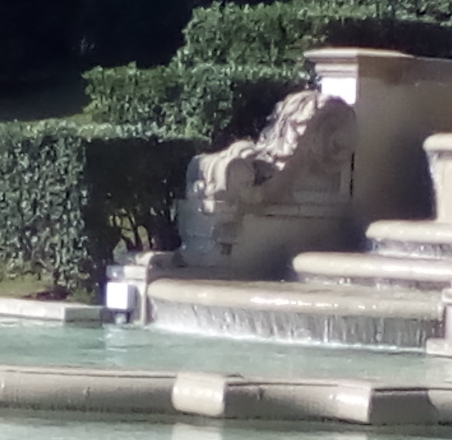
\includegraphics[height=1cm]{images/experiments/jardi_sel}
			%\hspace{0.1cm}
			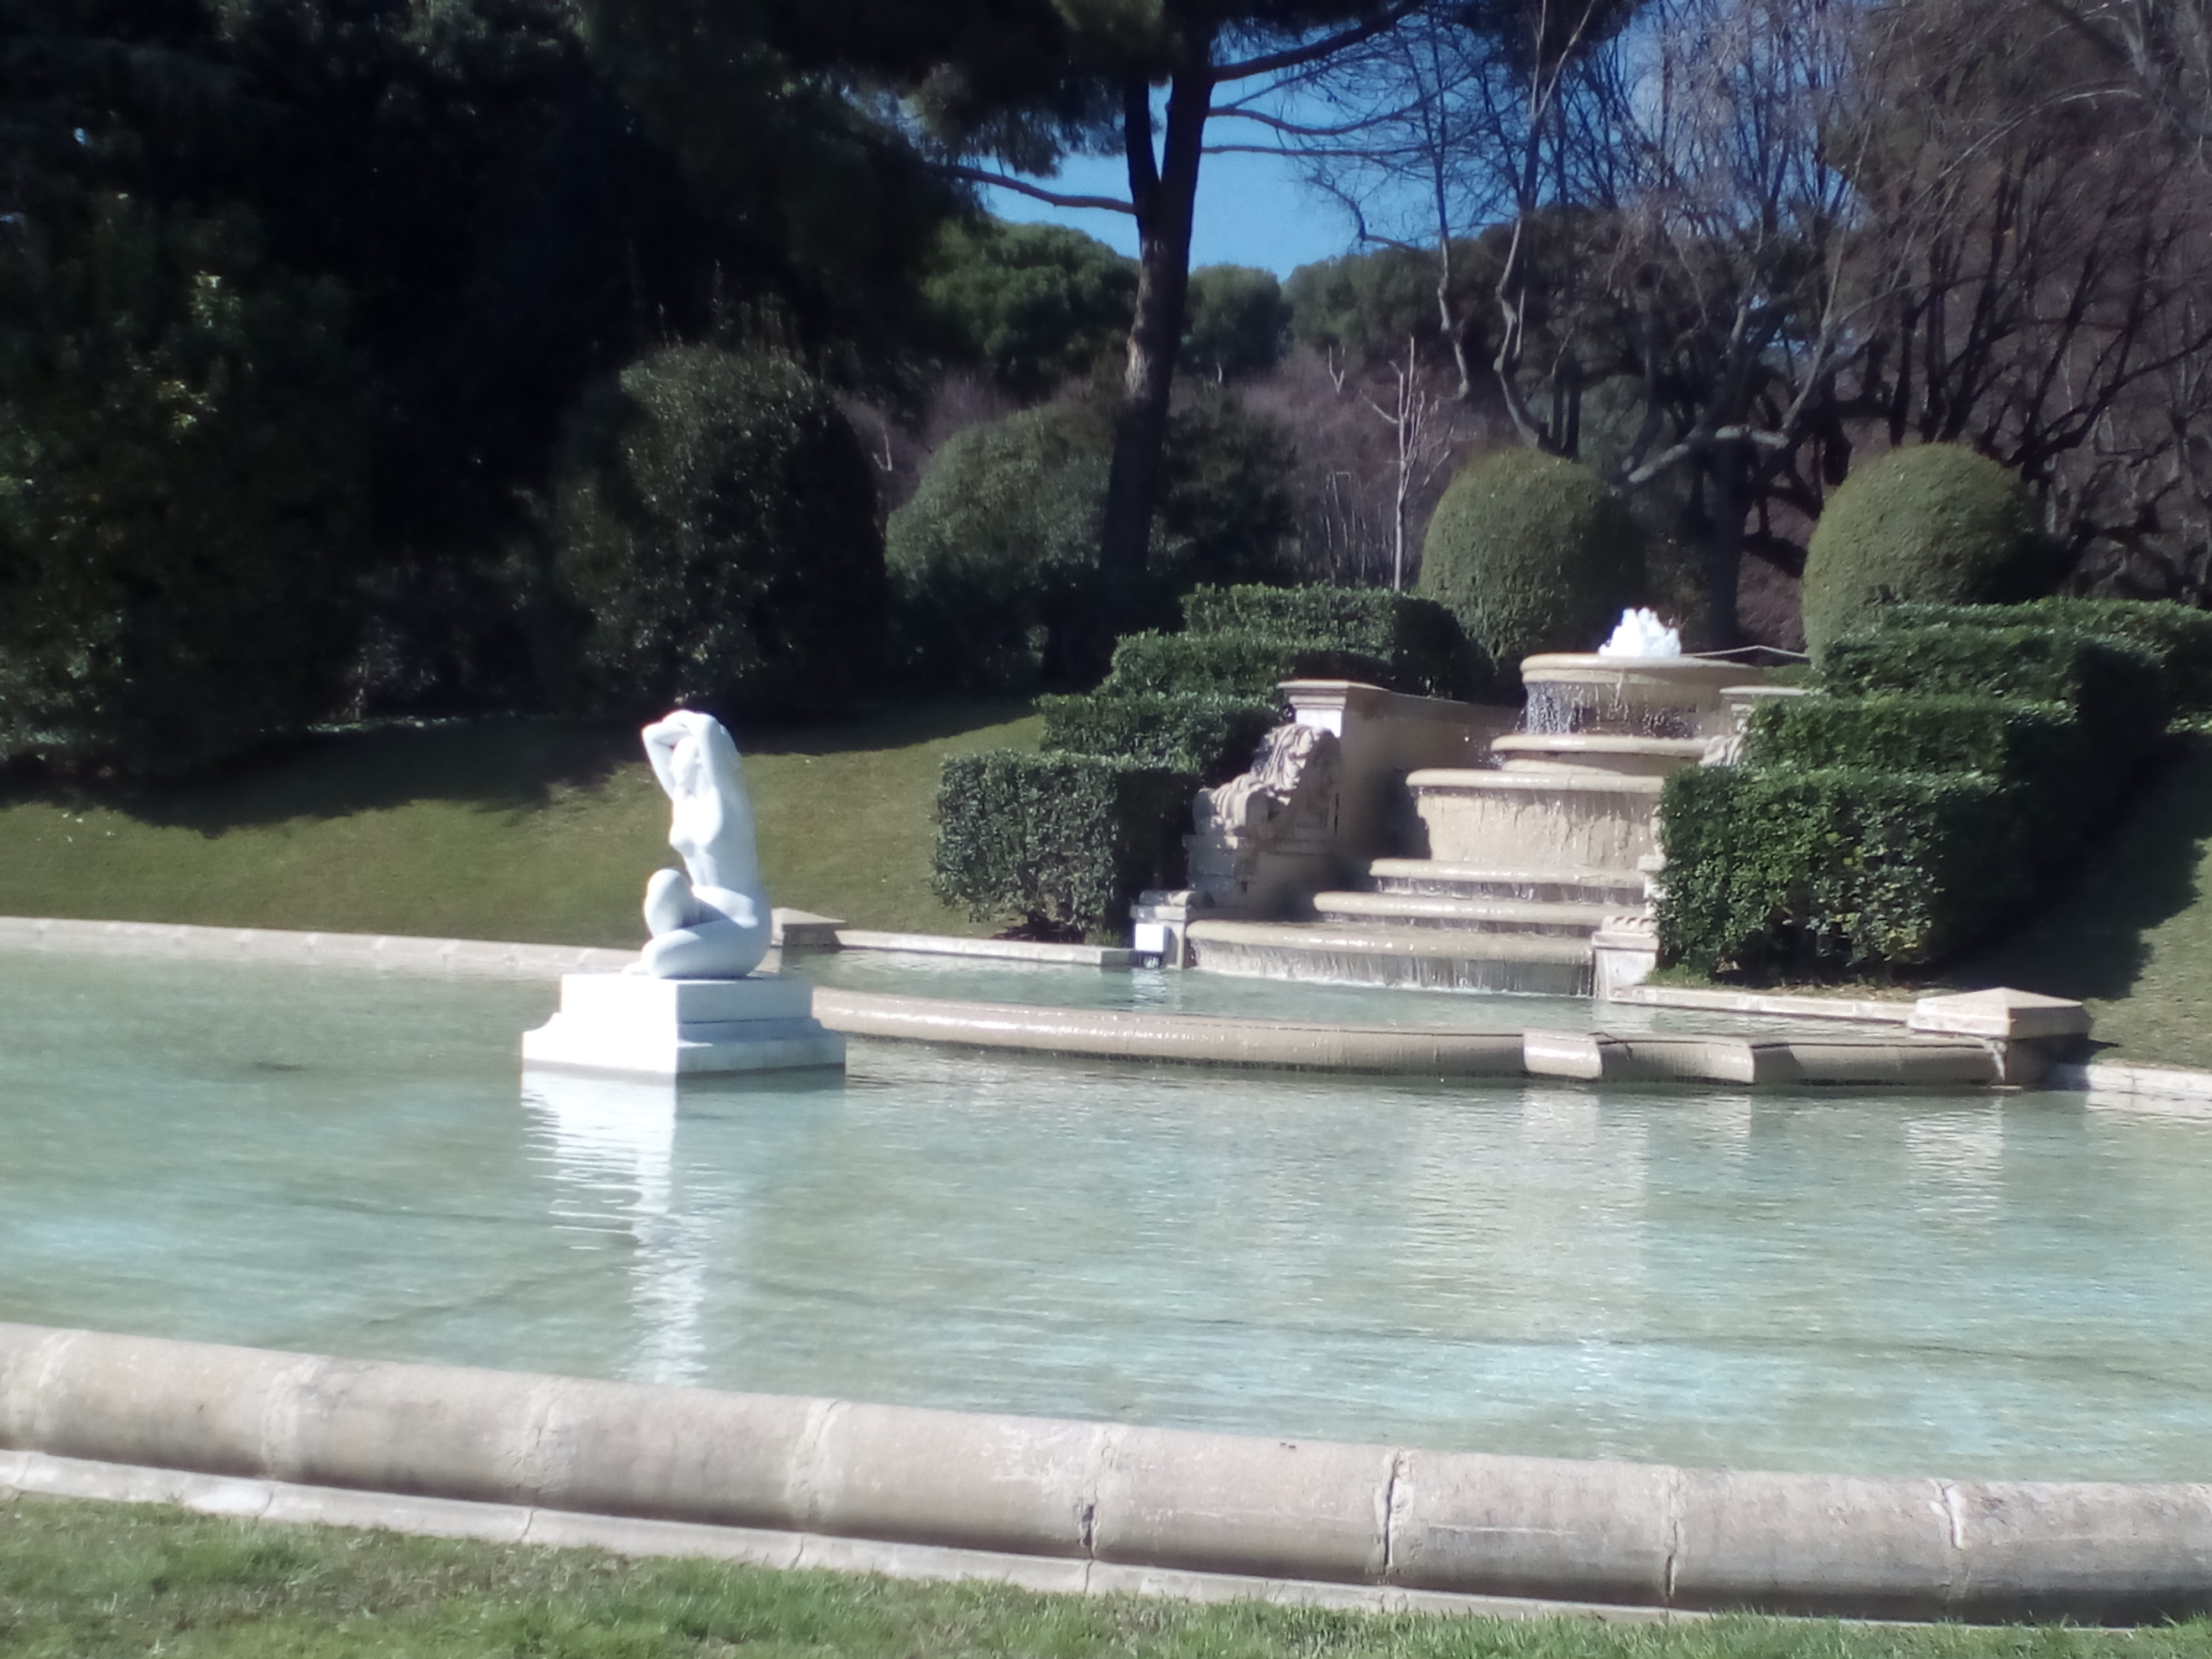
\includegraphics[height=1cm]{images/experiments/jardi_2}}
			\caption{Imatges campus i jardins palau reial}
		\end{figure}
	\end{frame}

	\begin{frame}{Objectes II}
		\tz
		\begin{table}[H]
			\begin{center}
				\rowcolors{3}{}{myBlue}
				\adjustbox{max width=\textwidth}{
				\begin{tabular}{l | c c | c c}
					& \multicolumn{2}{c|}{\textbf{Campus (moto)}} & \multicolumn{2}{c}{\textbf{Jardins (font)}} \\
					\textbf{Algorismes} & \textbf{Correctes} & \textbf{Erronis} & \textbf{Correctes} & \textbf{Erronis} \\ \hline
					Harris + SIFT & 30 & 0 & 38 & 0 \\
					SIFT + SIFT & 15 & 1 & 49 & 2 \\
					ORB + ORB & 14 & 1 & 52 & 10 \\
					ORB + BRISK & 19 & 0 & 71 & 6 \\
				\end{tabular}
				}
			\end{center}
			\caption{\textit{Matching} - objectes}
		\end{table}
	\end{frame}

	\begin{frame}{Imatges diferents I}
		\tz
		\begin{figure}[H]
			\resizebox{0.6\textwidth}{!}{%
			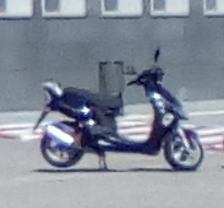
\includegraphics[height=1cm]{images/experiments/uni_sel}
			%\hspace{0.1cm}
			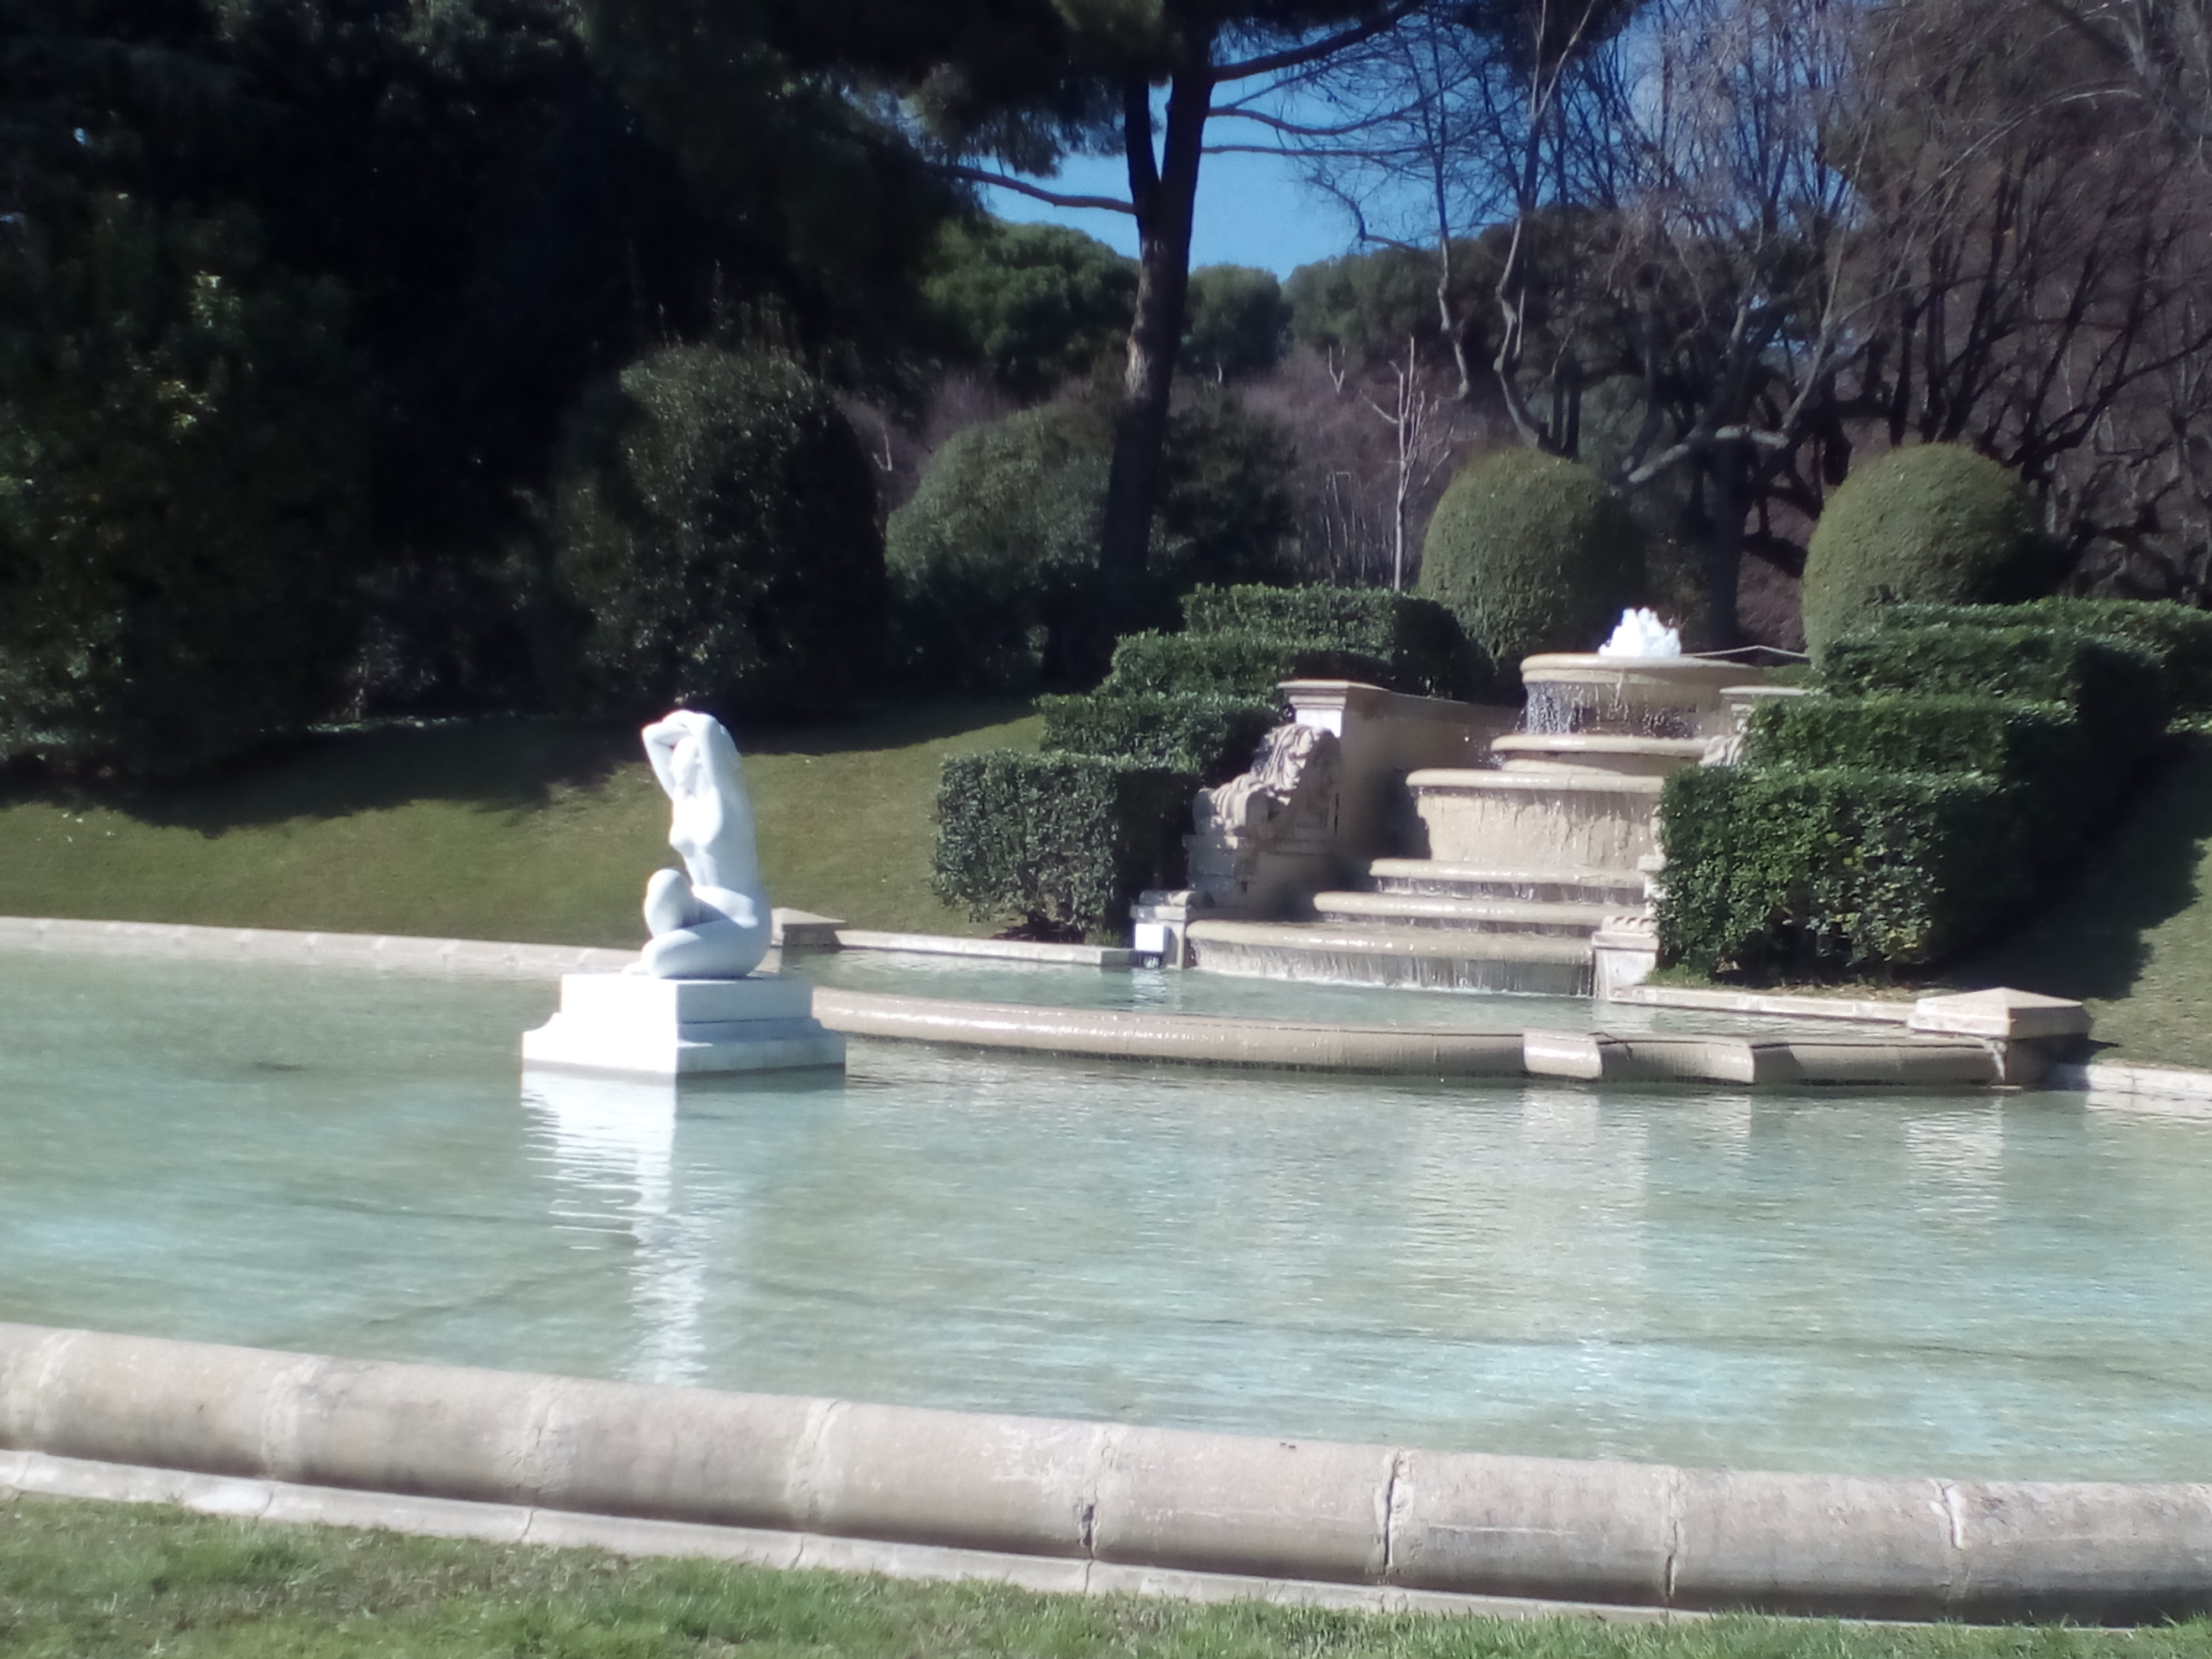
\includegraphics[height=1cm]{images/experiments/jardi_2}}
			%\vspace*{2cm}
			\par
			\resizebox{0.6\textwidth}{!}{%
			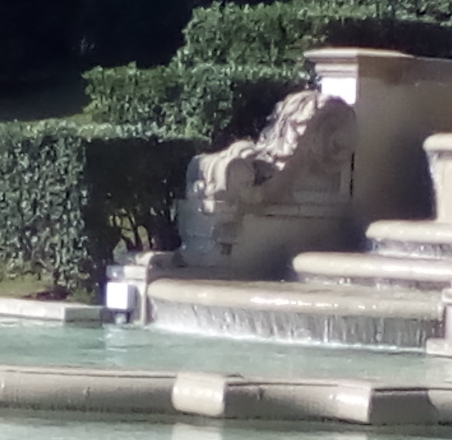
\includegraphics[height=1cm]{images/experiments/jardi_sel}
			%\hspace{0.1cm}
			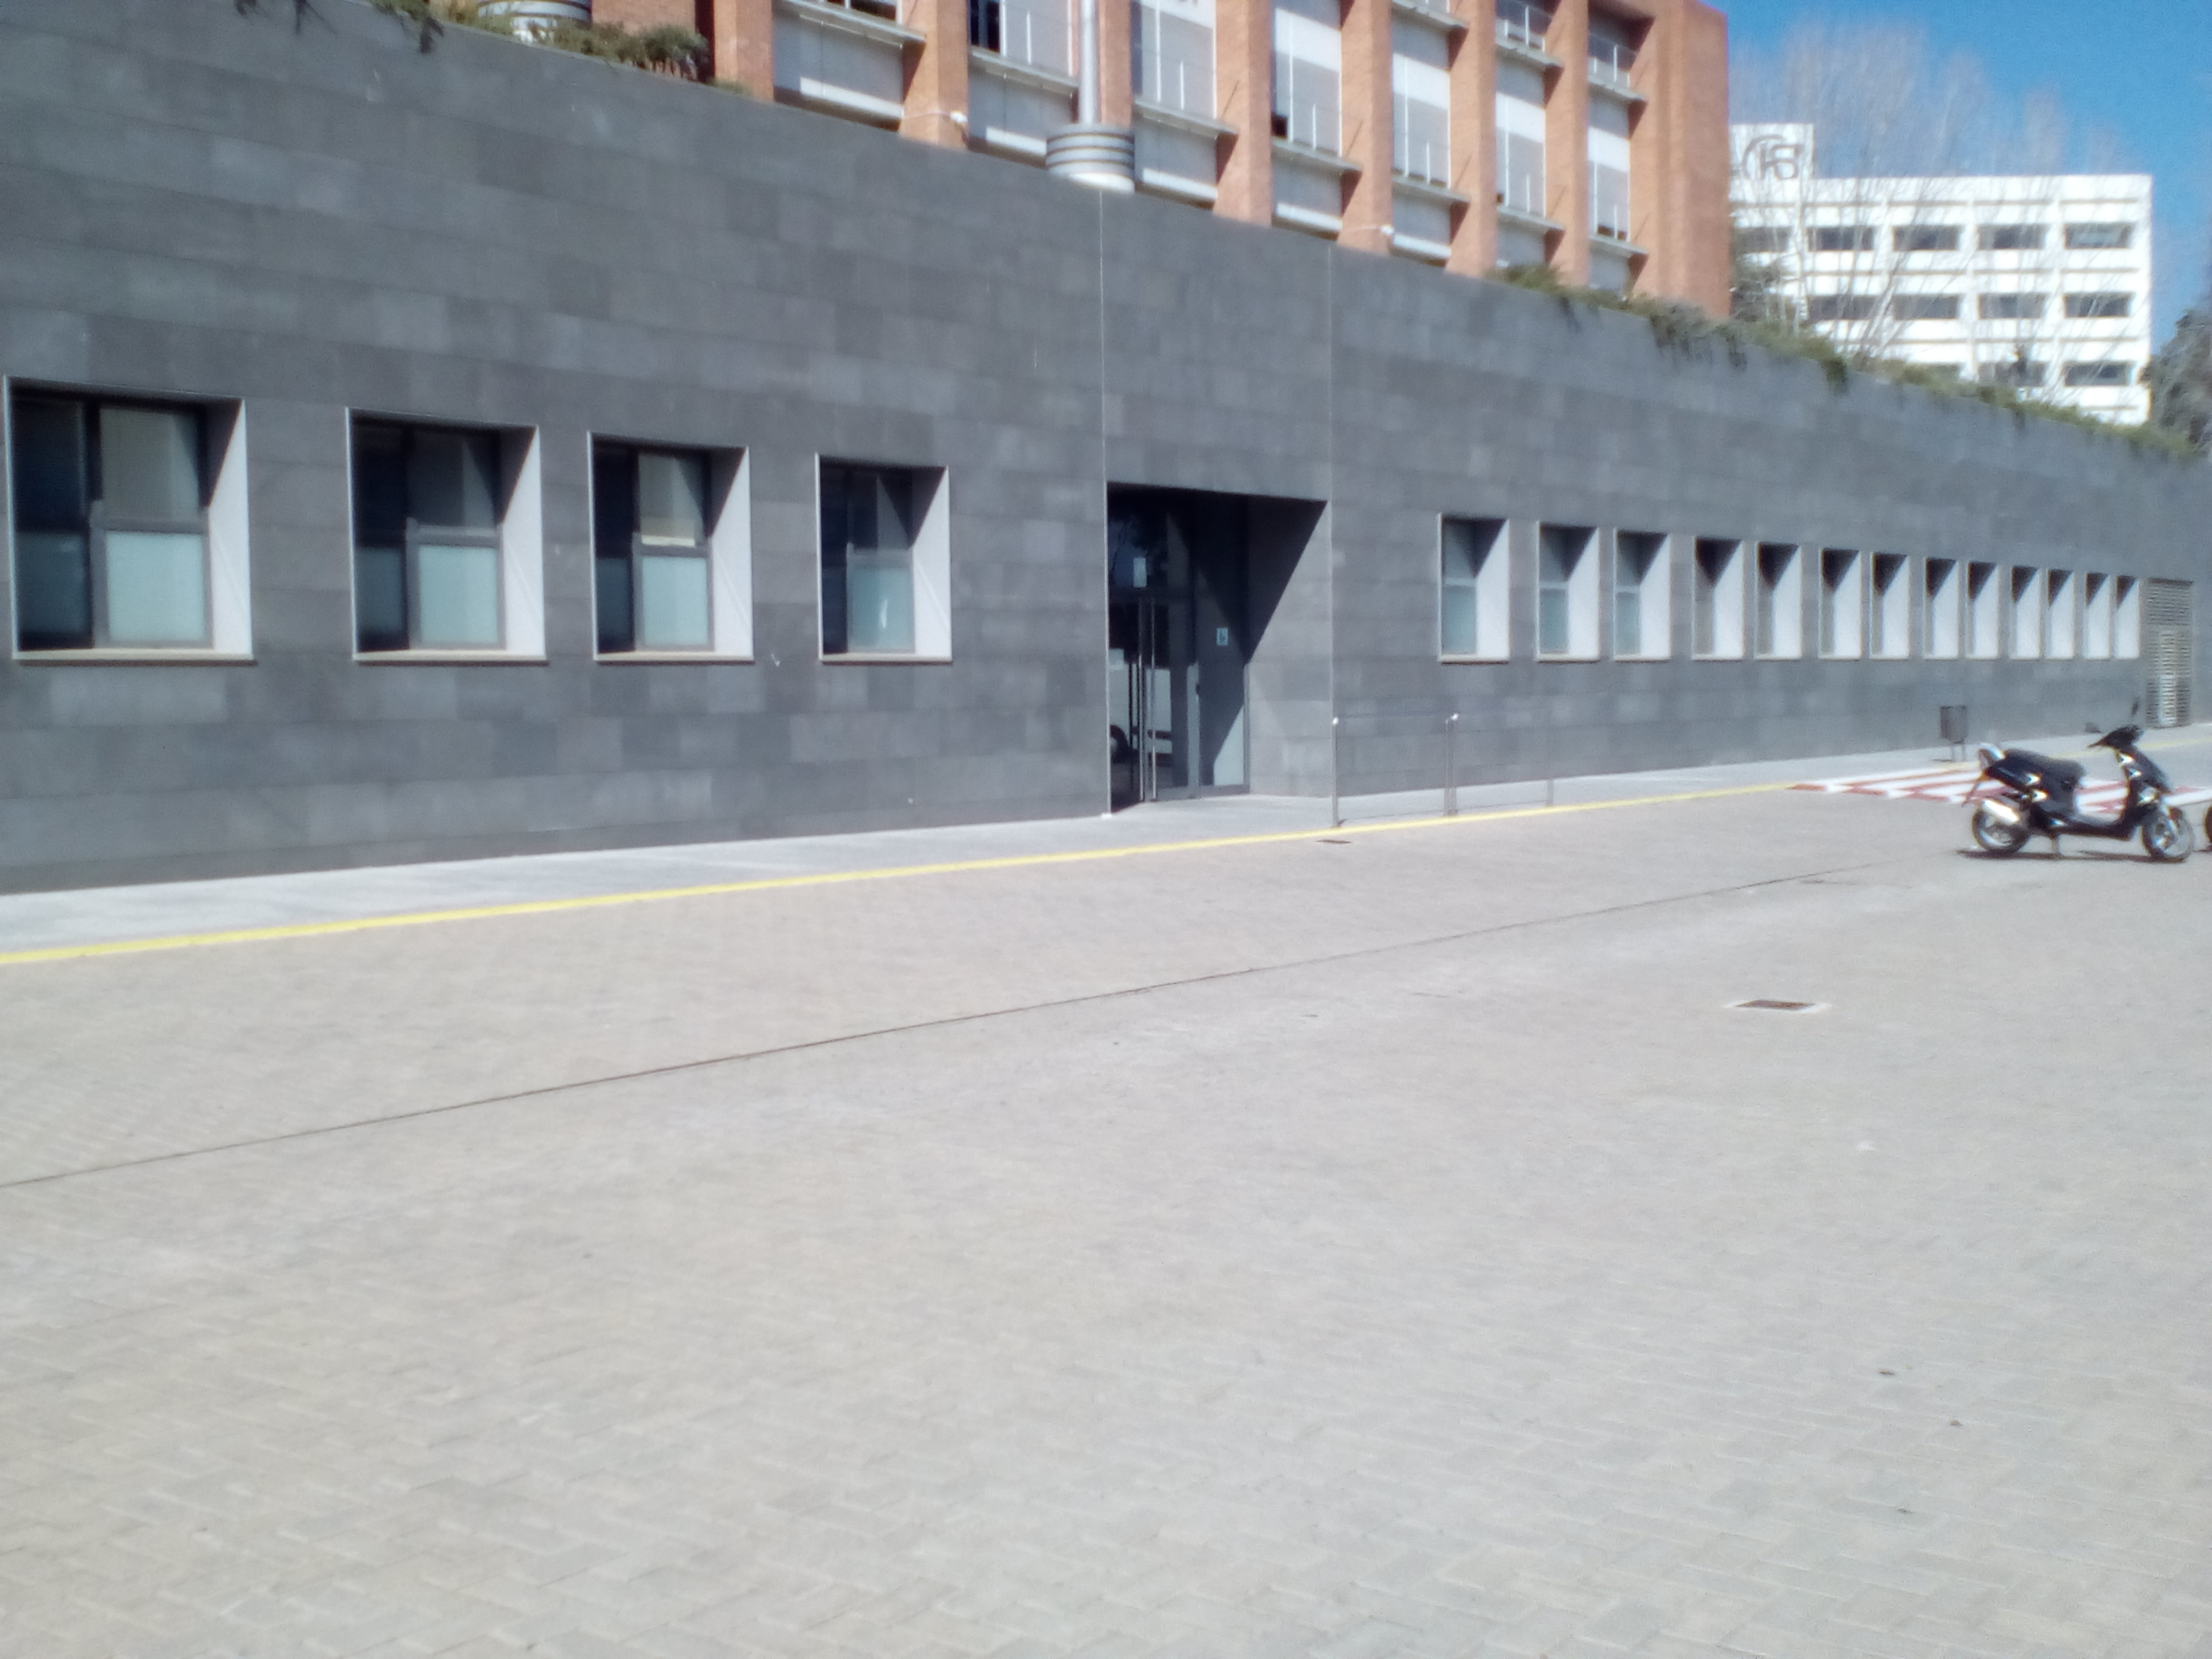
\includegraphics[height=1cm]{images/experiments/uni1}}
			\caption{Imatges campus i jardins palau reial}
		\end{figure}
	\end{frame}

	\begin{frame}{Imatges diferents II}
		\tz
		\begin{table}[H]
			\begin{center}
				\rowcolors{3}{}{myBlue}
				\adjustbox{max width=\textwidth}{
				\begin{tabular}{l | c c c c | c c c c}
					& \multicolumn{4}{c|}{\textbf{Set 1}} & \multicolumn{4}{c}{\textbf{Set 2}} \\
					\textbf{Algorismes} & \textbf{Kp1} & \textbf{Kp2} & \textbf{Parells} & \textbf{t} & \textbf{Kp1} & \textbf{Kp2} & \textbf{Parells} & \textbf{t} \\ \hline
					Harris + SIFT & 67 & 757 & 0 & 0.331s & 304 & 417 & 2 & 0.839s \\
					SIFT + SIFT & 125 & 5148 & 1 & 0.987s & 570 & 1342 & 5 & 1.113s \\
					ORB + ORB & 830 & 2500 & 2 & 0.840s & 2405 & 2500 & 7 & 0.113s \\
					ORB + BRISK & 830 & 2500 & 1 & 0.942s & 2405 & 2500 & 7 & 1.003s \\
				\end{tabular}
				}
			\end{center}
			\caption{\textit{Matching} - imatges diferents}
		\end{table}
	\end{frame}

	\begin{frame}{Resultats matching i homografia}
		\tz
		\begin{figure}[!htb]
			\resizebox{0.8\textwidth}{!}{%
			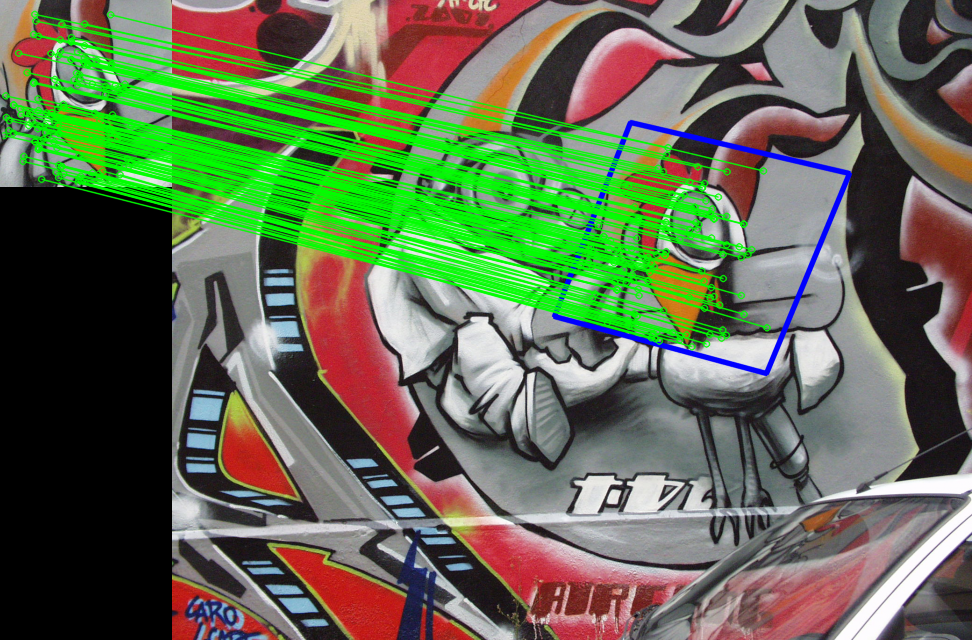
\includegraphics[height=1cm]{images/homography}
			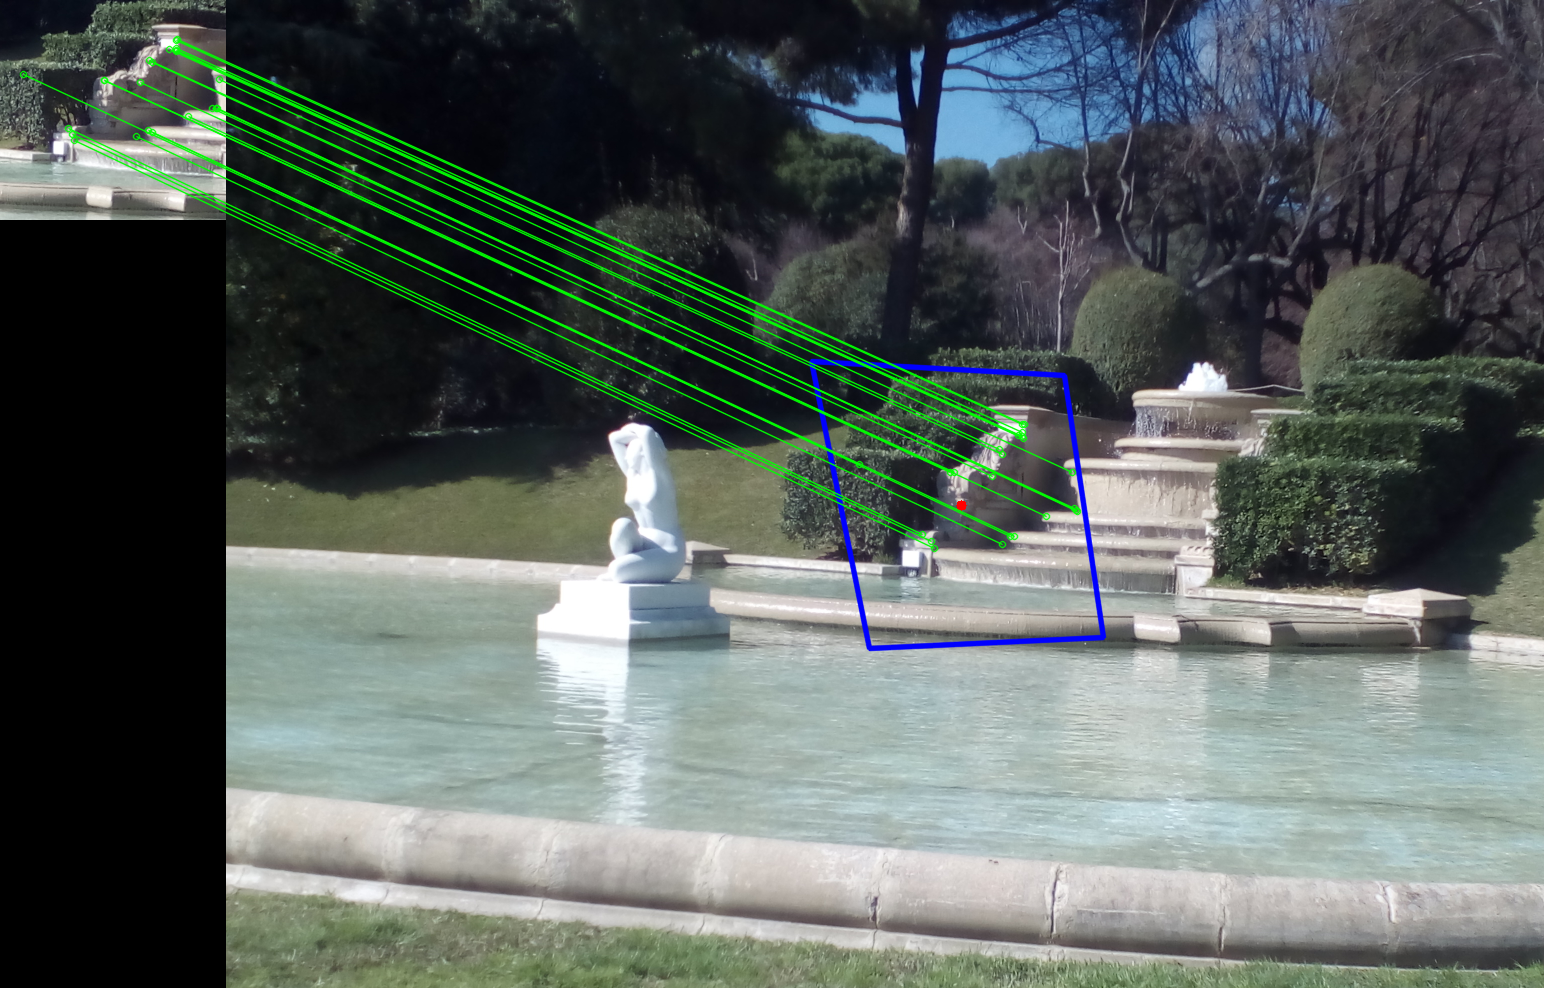
\includegraphics[height=1cm]{images/6}}
			\par
			\resizebox{0.8\textwidth}{!}{%
			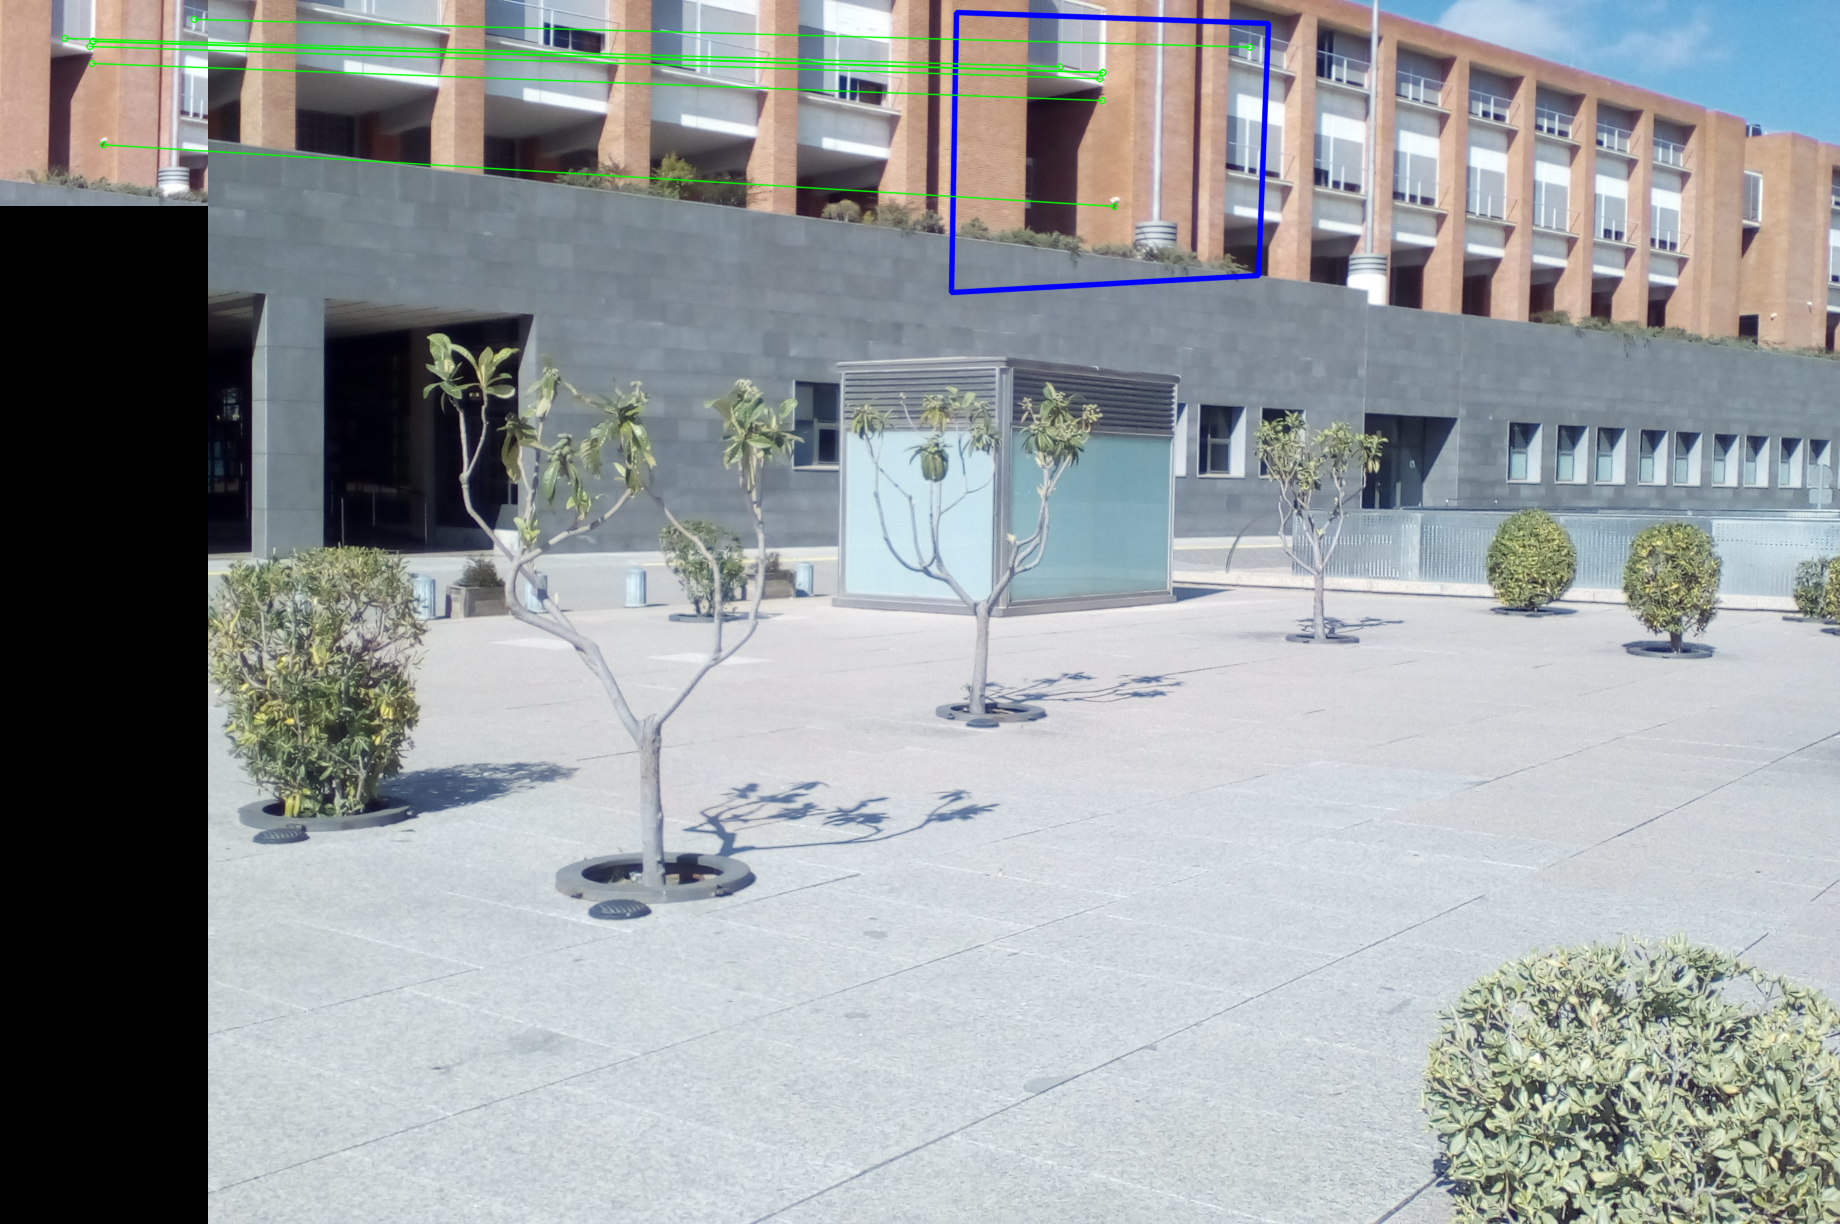
\includegraphics[height=1cm]{images/uniSel5}
			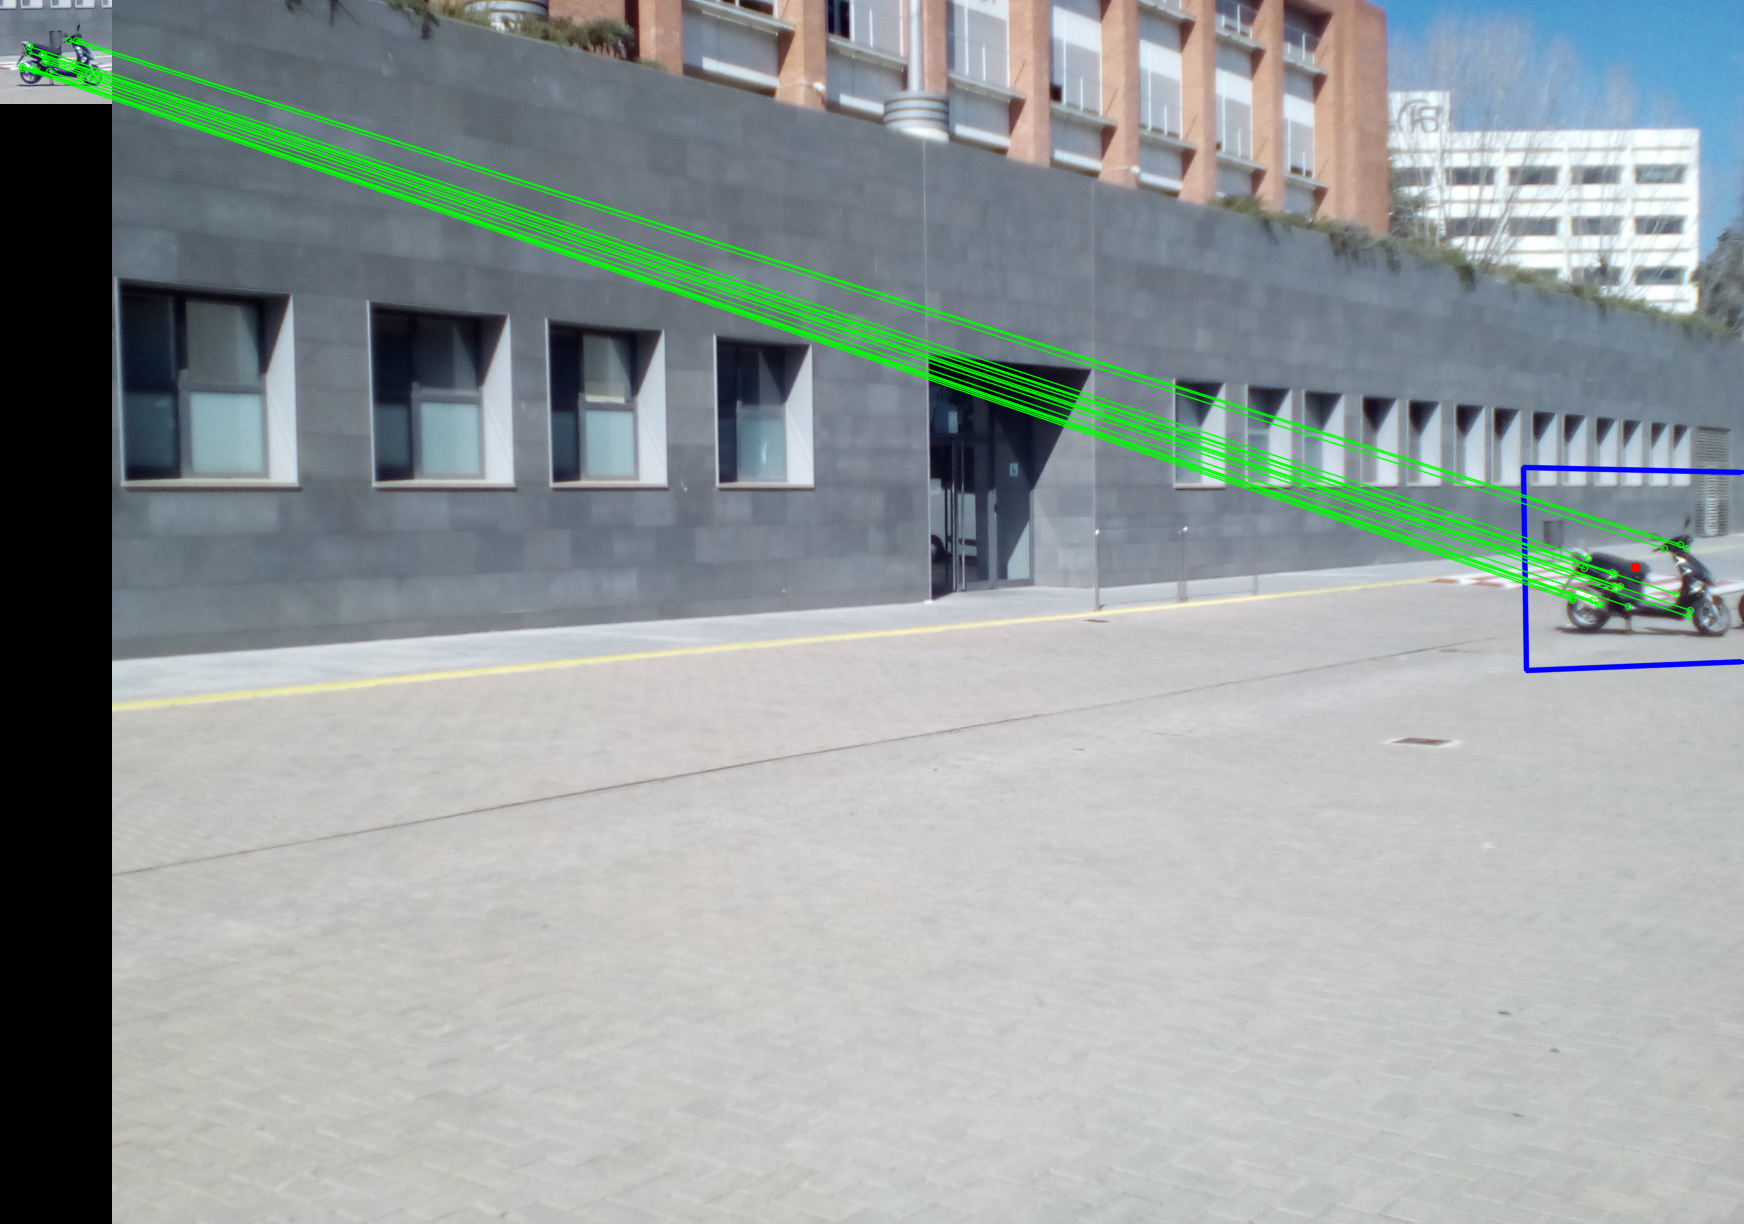
\includegraphics[height=1cm]{images/7}}
			\caption{Homografia - Resultats}
		\end{figure}
	\end{frame}


	\begin{frame}[plain]
		\section{Conclusions}
	\end{frame}

	\begin{frame}{Conclusions}
		\tz
		L'objectiu principal s'ha complert.
		\vspace{1em}

		\begin{itemize}
			\item Harris + SIFT més robust
			\item ORB alternativa ràpida
			\item Marge de millora
		\end{itemize}
	\end{frame}

	\begin{frame}{Treball futur}
		\tz
		\begin{itemize}
			\item{Comparació i anàlisi d'algorismes}
			\item{Diferents imatges}
			\item{Preprocessat}
			\item{Aplicació mòbil}
			\item{Entorn real + robot}
		\end{itemize}
	\end{frame}

	\begin{frame}[standout,plain]
		\Huge{Gràcies per la vostra\\atenció}
	\end{frame}

	\appendix

	\begin{frame}[allowframebreaks]{Referències}
		\printbibliography[heading=none]
	\end{frame}

\end{document}
